\documentclass[11pt]{article}
\usepackage[margin=2.54cm]{geometry}
\usepackage{amsfonts, amsmath, amssymb}
\usepackage{graphicx}
\graphicspath{ {images/} }
\usepackage[hidelinks]{hyperref}
\usepackage[polish, english]{babel}
\usepackage[shortlabels]{enumitem}
\usepackage[utf8]{inputenc}
\usepackage[T1]{fontenc}
\usepackage{float}
\setlength{\parindent}{0em}

\begin{document}

\thispagestyle{empty}
\tableofcontents
\clearpage
\setcounter{page}{1}

\section{Problem definition} \label{problem_definition}
Report on the alcoholic beverages market in Poland, performed by audit company KPMG \cite{kpmg_alco}, claims, that in 2013, Poles spent 41.1 billion zlotys on alcohol, with beer being a large portion of that amount (47\%). The report also states that, as of 2014, Polish customers choose beers based on premiumisation (31\% of customers), innovation (29\%) and region affiliations (30\%), with manufacturers predicting significant rise of interest in those attributes in the future. The evolution in customers' taste and their openness resulted in many local shops offering a vast range of, so called, "craft beers" coming from lesser known breweries. However, it's also not uncommon to stumble upon large product shelves, with dozens different beers types, in more popular Polish stores like Lidl and Carrefour.\\

\begin{figure}[h]
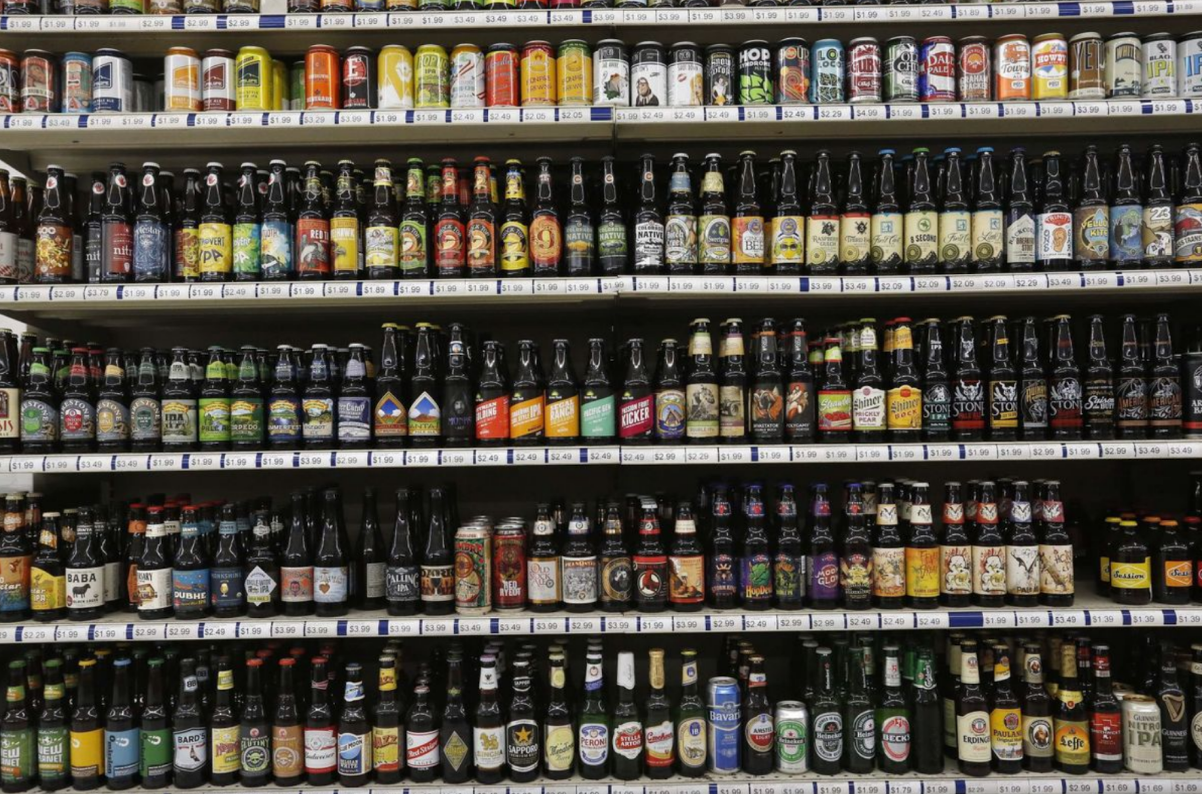
\includegraphics[width=0.5\textwidth]{beer_shelf}
\centering
\caption{A large beer shelf. Source: \protect \url{http://trib.com}.}
\label{fig:beer_shelf}
\end{figure}

The question this thesis posed at first was "How technology could be used to help a customer, who stands in front of a supermarket's large beer shelf (\autoref{fig:beer_shelf}.) and tries to choose one, not knowing anything about beers?". The answer appeared to be relatively simple and involved developing a mobile application, which could connect to beer database residing in Cloud e. g. Firebase Realtime Database and retrieve details about any given beer. The real problem, that later emerged, and is in fact the basis of this thesis, is "Given a mobile application, that can connect to beer database in Cloud, what is the most intuitive, appealing and fastest way of accessing this database from the device?".
\clearpage

\section{Solution overview} \label{solution_overview}
To further investigate the problem articulated in Chapter \ref{problem_definition}, a survey was conducted \cite{survey}. Its main question was "Imagine standing in front of a big shelf with hundreds of craft beers you've never seen before. There's no one there to help you except a mobile app with beer database, which you can access in different ways: typing beer name, using voice to input beer name, making photo of front beer label, making photo of bar code in the back of the bottle. Rank those ways starting from the one that's the most intuitive and appealing to you.". Interestingly, the most popular option, among 50 people asked, was making a photo of front beer label. This method of database access was almost equally popular to the most standard human-device communication interface, which is keyboard (typing a beer name). Whereas \autoref{fig:survey_chart} presents the overall trend, \autoref{fig:survey_table} provides us with detailed numbers: 60\% of people chose, in either first or second place, making a photo of front beer label as their preference (same as in typing a beer name by hand). The last thing that's worth noting is the lack of popularity of barcode scanning.\\

Based on the aforementioned survey and personal experience, a solution to the problem, stated in Chapter \ref{problem_definition}, was formulated as a design and implementation of server-client recognition system for beer labels.

\begin{figure}[h]
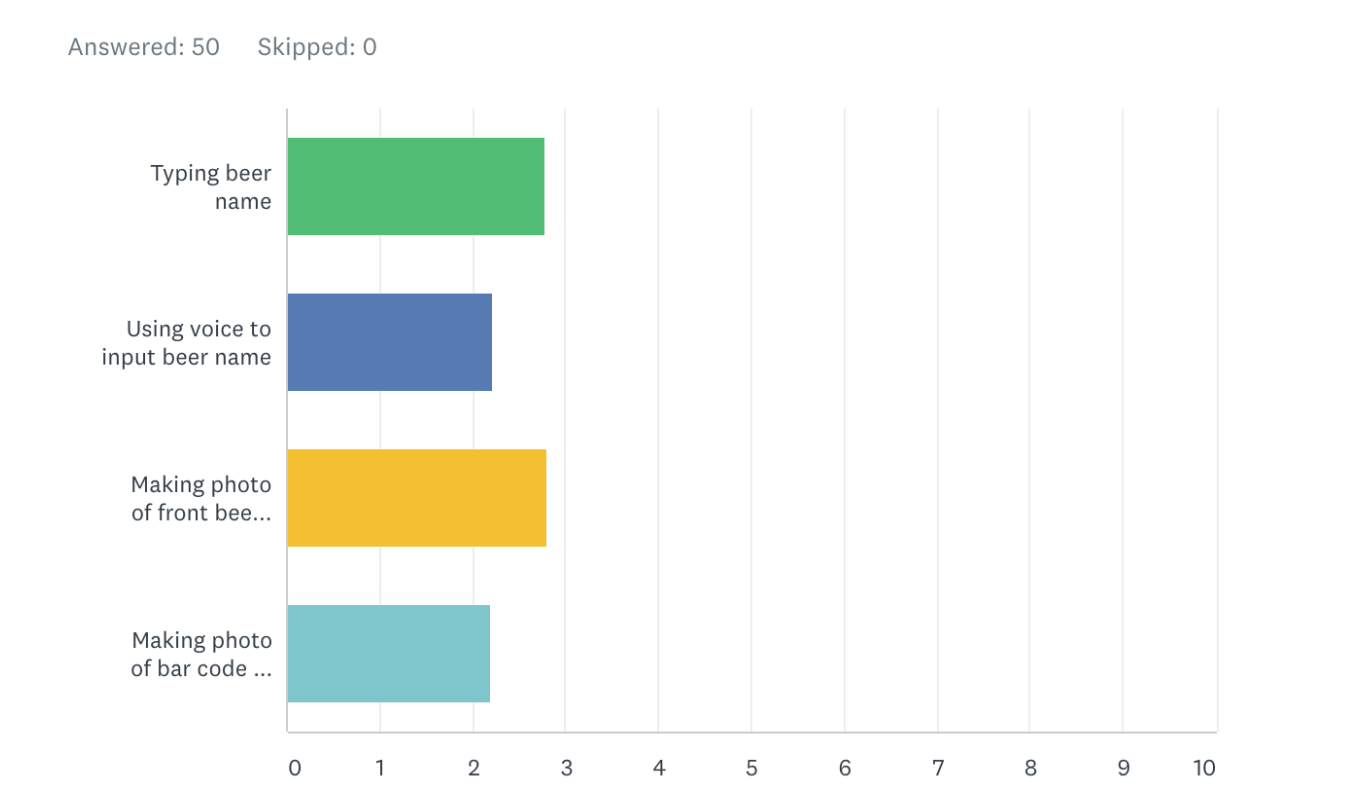
\includegraphics[width=0.8\textwidth]{survey_chart}
\centering
\caption{Weighted average of respondents' answers (chart). For choosing an option as first - weight: 4, for choosing an option as second - weight: 3 etc. Obtained sum is then divided by total number of respondents (here: 50).}
\label{fig:survey_chart}
\end{figure}

The goal of this section is to give a reader, in a few short points, an overall idea of the recognition system before theoretical introduction. Chapter \ref{solution_walkthrough} focuses on implementation details. \autoref{fig:scheme} presents a scheme with a functional principle of implemented server-client beer label recognizer, namely:
\begin{enumerate}
\item An image of beer label is taken by the Android \cite{android_guide} application. 
\item Android application sends the image to the Flask \cite{flask_docs} server equipped with algorithm, which performs beer label prediction.
\item Encoded prediction is returned to Android application.
\item Encoded prediction is used as a key to the beer database residing in Firebase Cloud \cite{firebase_database_docs}.
\item Based on the key (encoded label name) all information about given beer is sent to Android application and displayed to the user.
\end{enumerate}

\begin{figure}[h]
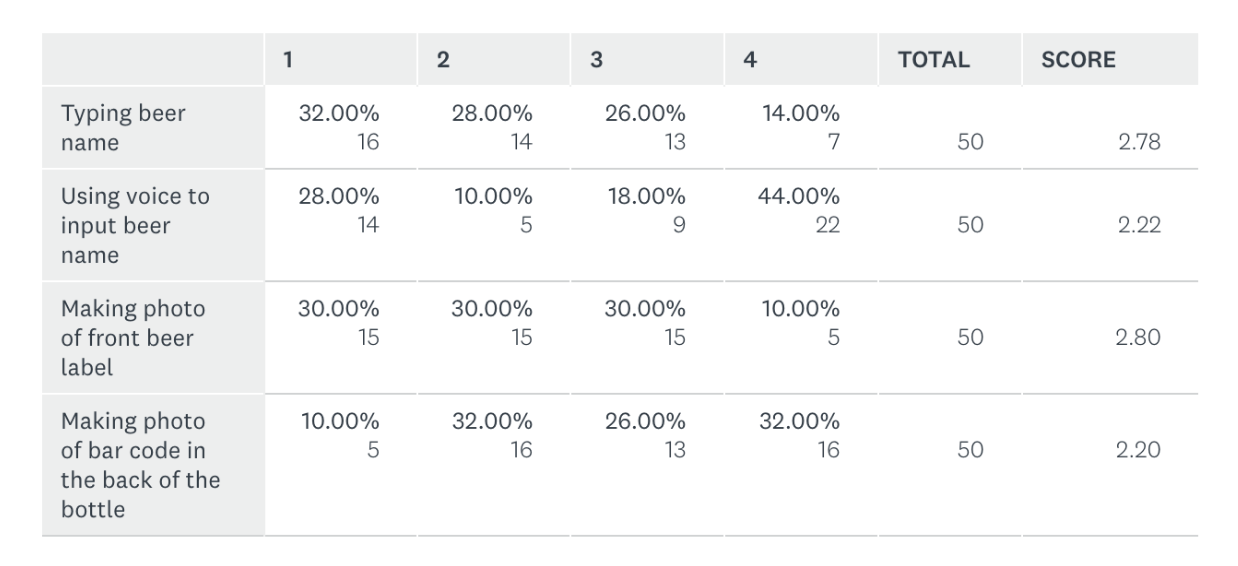
\includegraphics[width=0.8\textwidth]{survey_table}
\centering
\caption{Weighted average of respondents' answers (table with details). For method of average calculation see: \autoref{fig:survey_chart}.}
\label{fig:survey_table}
\end{figure}

\begin{figure}[h]
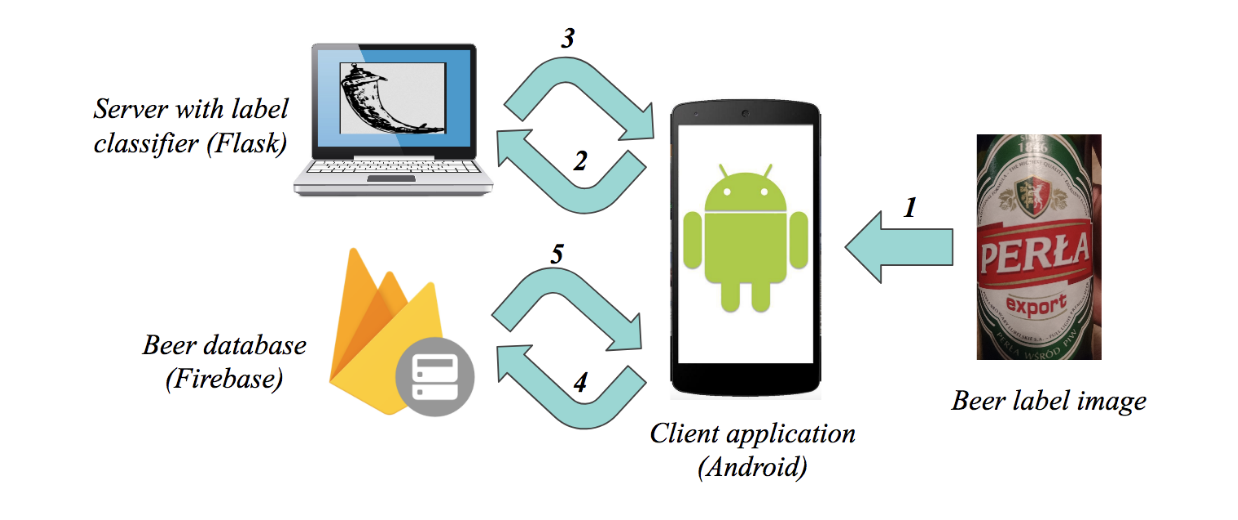
\includegraphics[width=0.8\textwidth]{scheme}
\centering
\caption{Server-client recognition system for beer labels with functional principle (consecutive steps enumerated).}
\label{fig:scheme}
\end{figure}
\clearpage

\section{Introduction to Artificial Intelligence} \label{introduction_to_ai}
There are many approaches to define Artificial Intelligence (AI), but perhaps the most famous is the one formed by Alan Turing in 1950. The proposed method, referred to as Turing test, involved human subject asking written questions to a computer and receiving written answers. If the interrogator couldn't tell if responses came from a human or a machine - the test was passed, i. e. the computer was considered intelligent (at least in some sense). Even stricter rules were imposed on conduction of, so called, total Turing test. In addition to requirements mentioned previously, a computer needed to fool a human subject through a proper visual perception and human-like object manipulations (robotics).\\

Achieving a feat of passing either of aforementioned tests requires multidisciplinary knowledge in many fields. Norvig and Russell \cite{ai_modern_approach} did a remarkable job of listing major disciplines, that contributed to the growth of AI, namely:
\begin{enumerate}[a)]
\item philosophy,
\item mathematics,
\item economics,
\item neuroscience,
\item psychology,
\item computer engineering,
\item control theory and cybernetics,
\item linguistics.
\end{enumerate}
Despite invaluable contributions from greatest minds in above fields, the Holy Grail of some researchers - Artificial General Intelligence, often called "strong AI", capable of performing any intellectual task of human being - is still far ahead. Focus of many scientists, and also of this thesis, is, conversely, on creating algorithm, which behaves in an intelligent manner in a specific area of expertise (e. g. computer vision), but fails miserably in others (e. g. voice recognition). A big part of this approach revolves around a branch of Artificial Intelligence called supervised learning. \\

In essence, supervised learning is inference of correct outputs from given inputs based on labeled training set. Examples of this include:
\begin{enumerate}[a)]
\item given an email, is it spam or not?
\item given an image, does it contain face or not?
\item given an audio clip, what is the correct transcript?
\item given a Polish sentence, what is semantically correct English translation?
\item given a beer label image, what is the name of the beer?
\end{enumerate}
Prerequisites of performing such tasks are, usually, a large amount of data (e. g. actual emails correctly marked as spam or not) and big computational power (powerful Graphics Processing Units, High-Performance Computing), both of which significantly increased over the past years (\autoref{fig:cpu_gpu}, \autoref{fig:cisco_era}).\\

\begin{figure}[h]
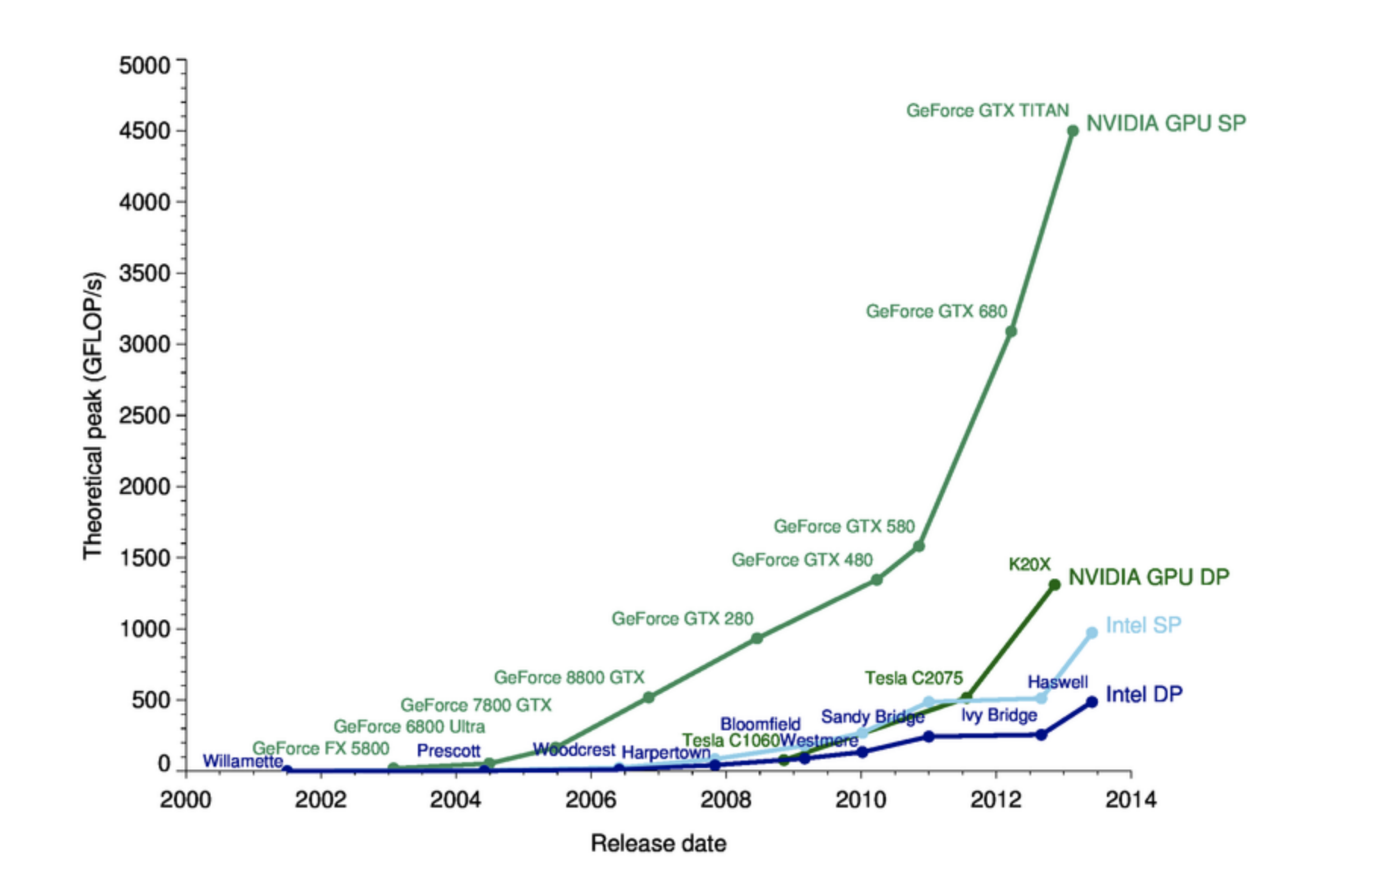
\includegraphics[width=0.75\textwidth]{cpu_gpu}
\centering
\caption{Performance of NVIDIA GPUs and Intel CPUs measured in GFLOP/s \cite{cpu_vs_gpu}.}
\label{fig:cpu_gpu}
\end{figure}

\begin{figure}[h]
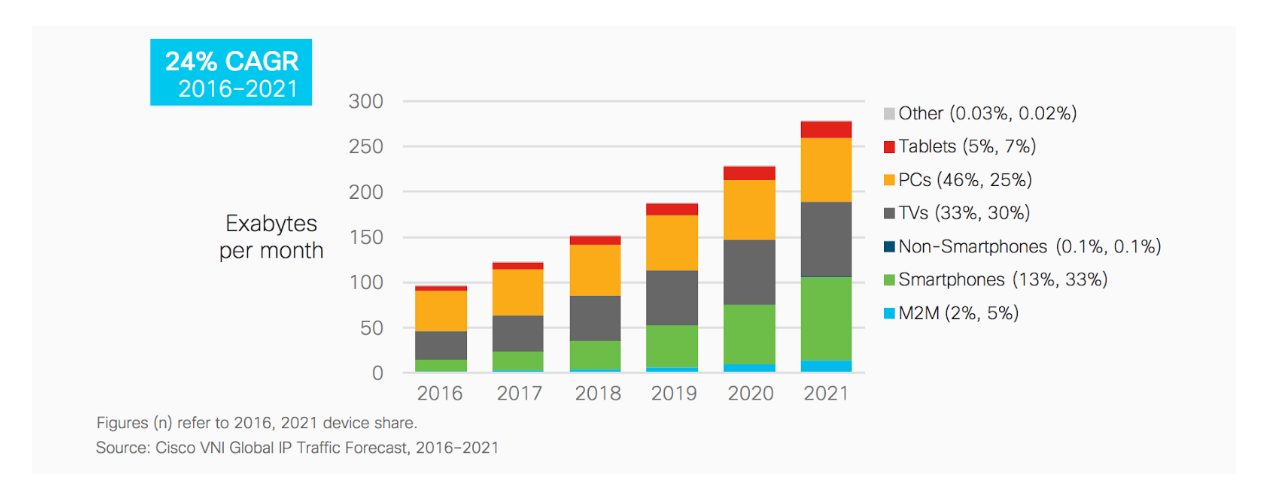
\includegraphics[width=0.8\textwidth]{cisco_era}
\centering
\caption{Global IP traffic by devices \cite{cisco_era} with 24\% compound annual growth rate (2016-2021).}
\label{fig:cisco_era}
\end{figure}

It is important to distinguish between Machine Learning (ML) and Artificial Intelligence. The former is considered to be a subset of the latter. Whereas AI comprises of knowledge base systems, genetic algorithms, Bayesian statistics etc., none of that is considered ML. Machine Learning can be defined as an act of optimization along a certain dimension (e. g. minimizing the error of choosing a wrong prediction of a beer label based on an image) and a primary tool for that is an algorithm called neural network, loosely based on a human brain cell.
\clearpage

\section{Introduction to Neural Networks} \label{introduction_to_nn}
It's reasonable to think of a neural network (NN) as a mathematical function, which in practice tends to be very complicated because of three things:
\begin{enumerate}[1)]
\item it has a large number of coefficients (weights), often exceeding tens of millions,
\item it's a very deeply nested function, hence even simple gradient calculation (partial derivative) is relatively slower,
\item most of its computations are performed on multidimensional tensors.
\end{enumerate}
\autoref{fig:no_activation_net} contains a popular representation of a simple neural network with three basic building blocks: unit (single circle with value $in_i^{(k)}$, input $x_i$, output $\hat{y_i}$ or bias $1$), layer (units arranged into one vertical group $k$) and weight (connection between units with value $w_{ij}^{(k)}$ representing its strength). \autoref{eq:y_hat_1}, \ref{eq:y_hat_2}, \ref{eq:in_1}, \ref{eq:in_2} and \ref{eq:in_3} translate this graphical representation to mathematical formula.\\

\begin{figure}[h]
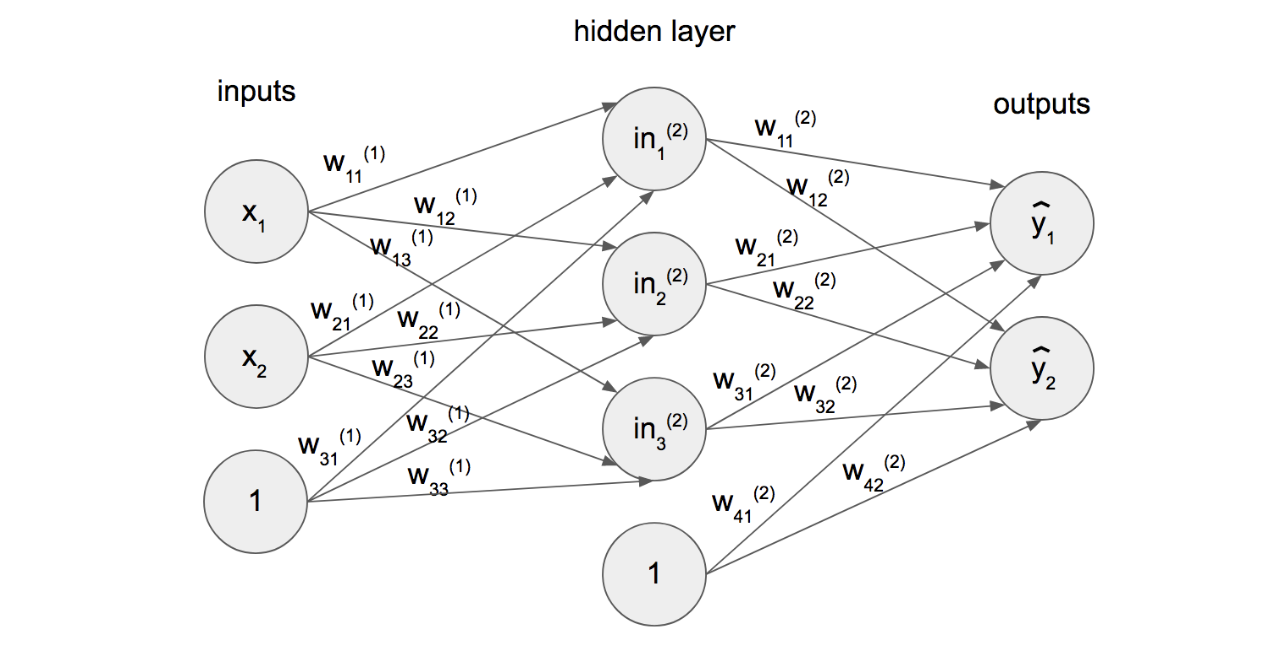
\includegraphics[width=0.8\textwidth]{no_activation_net}
\centering
\caption{A simple neural network with one hidden layer (a layer between inputs and outputs).}
\label{fig:no_activation_net}
\end{figure}

\begin{equation} \label{eq:y_hat_1}
\hat{y_1} = w_{11}^{(2)}in_1^{(2)} + w_{21}^{(2)}in_2^{(2)} + w_{31}^{(2)}in_3^{(2)} + w_{41}^{(2)} * 1 
\end{equation}

\begin{equation} \label{eq:y_hat_2}
\hat{y_2} = w_{12}^{(2)}in_1^{(2)} + w_{22}^{(2)}in_2^{(2)} + w_{32}^{(2)}in_3^{(2)} + w_{42}^{(2)} * 1 
\end{equation}

\begin{equation} \label{eq:in_1}
in_1^{(2)} = w_{11}^{(1)}x_1 + w_{21}^{(1)}x_2 + w_{31}^{(1)} * 1 
\end{equation}

\begin{equation} \label{eq:in_2}
in_2^{(2)} = w_{12}^{(1)}x_1 + w_{22}^{(1)}x_2 + w_{32}^{(1)} * 1 
\end{equation}

\begin{equation} \label{eq:in_3}
in_3^{(2)} = w_{13}^{(1)}x_1 + w_{23}^{(1)}x_2 + w_{33}^{(1)} * 1 
\end{equation}

"Perceptron" is a common name for a neural network, where inputs are immediately coupled with outputs (no hidden layers, unlike in \autoref{fig:no_activation_net}). The presence of hidden (middle) layer of units, which prevents from direct connections between inputs and outputs, allows neural network to model highly nonlinear mathematical functions. Norvig and Russell justify that, using XOR gate as an example, in a following manner: "[...] linear classifiers [...] can represent linear decision boundaries in the input space. This works fine for the carry function, which is a logical AND [...]. The sum function, however, is an XOR (exclusive OR) of the two inputs. [...] this function is not linearly separable so the perceptron cannot learn it. The linearly separable functions constitute just a small fraction of all Boolean functions." \cite{ai_modern_approach}\\

Before delving into learning process of NNs, it's important to make two additions to previous model:
\begin{enumerate}[1)]
\item error function (also called cost function),
\item activation function.
\end{enumerate}
Ad 1. The most reliable way for the algorithm to represent predictions is through a vector of probabilities. Consider an example of beer name predictions based on image of label. \autoref{fig:probability_vectors} shows a probability output of a classifier (notice that all values sum to 1), compared with an output, that it should strive for. A cost function, introduced in this section, called categorical cross entropy (\autoref{eq:cross_entropy}), simply measures the correlation between those two probability distributions (predicted and ideal). Notice that multiplication by one-hot encoded examples, forces the function to only compare non-zero elements of ideal distribution, with respective values of classifier output further from 1 being penalized more than values close to 1 (thanks to the nature of logarithm).\\ 

\begin{figure}[h]
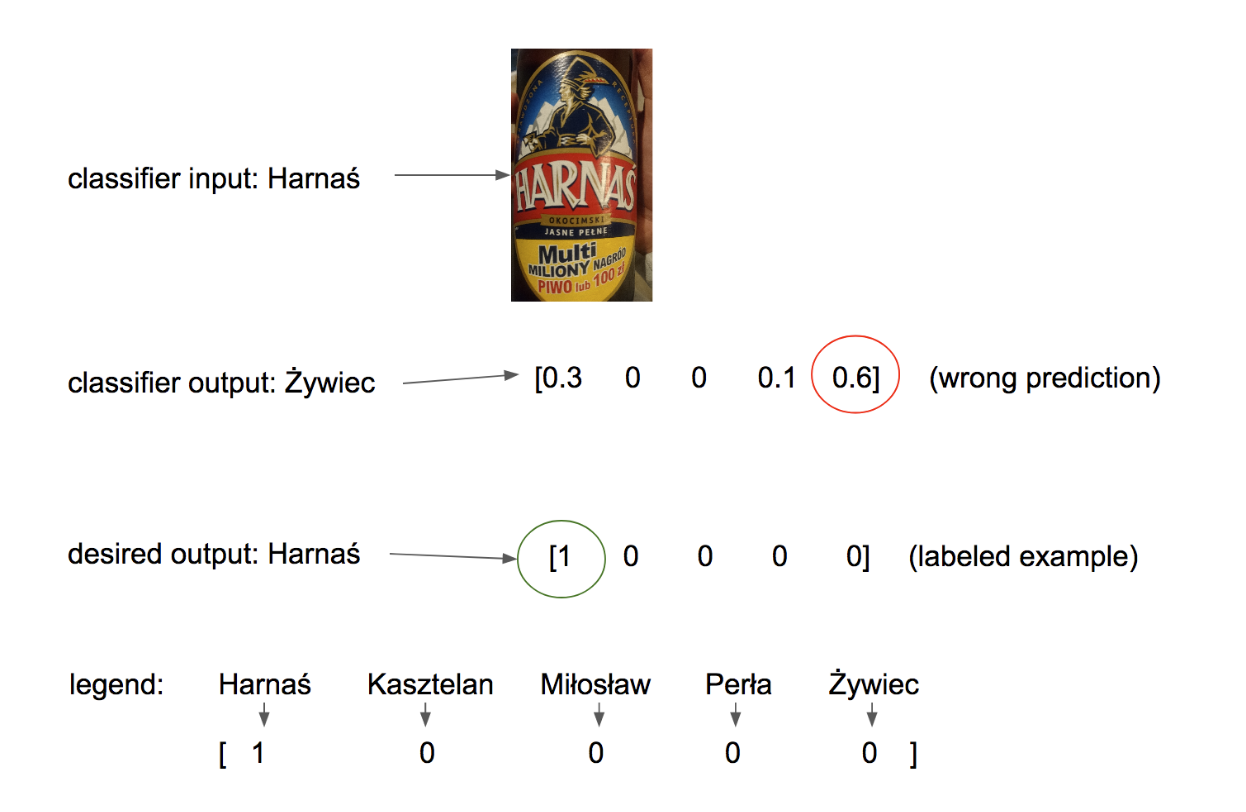
\includegraphics[width=0.8\textwidth]{probability_vectors}
\centering
\caption{Exemplary classifier input, output and desired (one-hot encoded) output with legend.}
\label{fig:probability_vectors}
\end{figure}

\begin{equation} \label{eq:cross_entropy}
H(d, p) = -\sum_i d_i * log(p_i)
\end{equation}
where:
\begin{itemize}
\item[$d_i$] is the $i^{th}$ element of one-hot encoded (desired) probability vector $d$,
\item[$p_i$] is the $i^{th}$ element of probability vector $p$ predicted by the classifier.
\end{itemize}

Ad 2. Unit's value $in_i^{(k)}$ is rarely propagated explicitly to next layers. So called activation function is used instead. The one I'll be introducing in this section is called sigmoid (\autoref{eq:sigmoid}). The updated model of simple neural network from \autoref{fig:no_activation_net} is shown in \autoref{fig:activation_net}. One thing worth pointing out is a difference between sigmoid and softmax function (\autoref{eq:softmax}) - both used in artificial neural networks. Whereas sigmoid inputs a single value and outputs a normalized scalar, softmax inputs a list of values and outputs a vector of real numbers in range [0, 1] that add up to 1, thus can be interpreted as a probability distribution. Sigmoid is used in hidden units, while softmax is usually applied in the last output layer. Both functions can be categorized as logistic functions.\\

\begin{figure}[h]
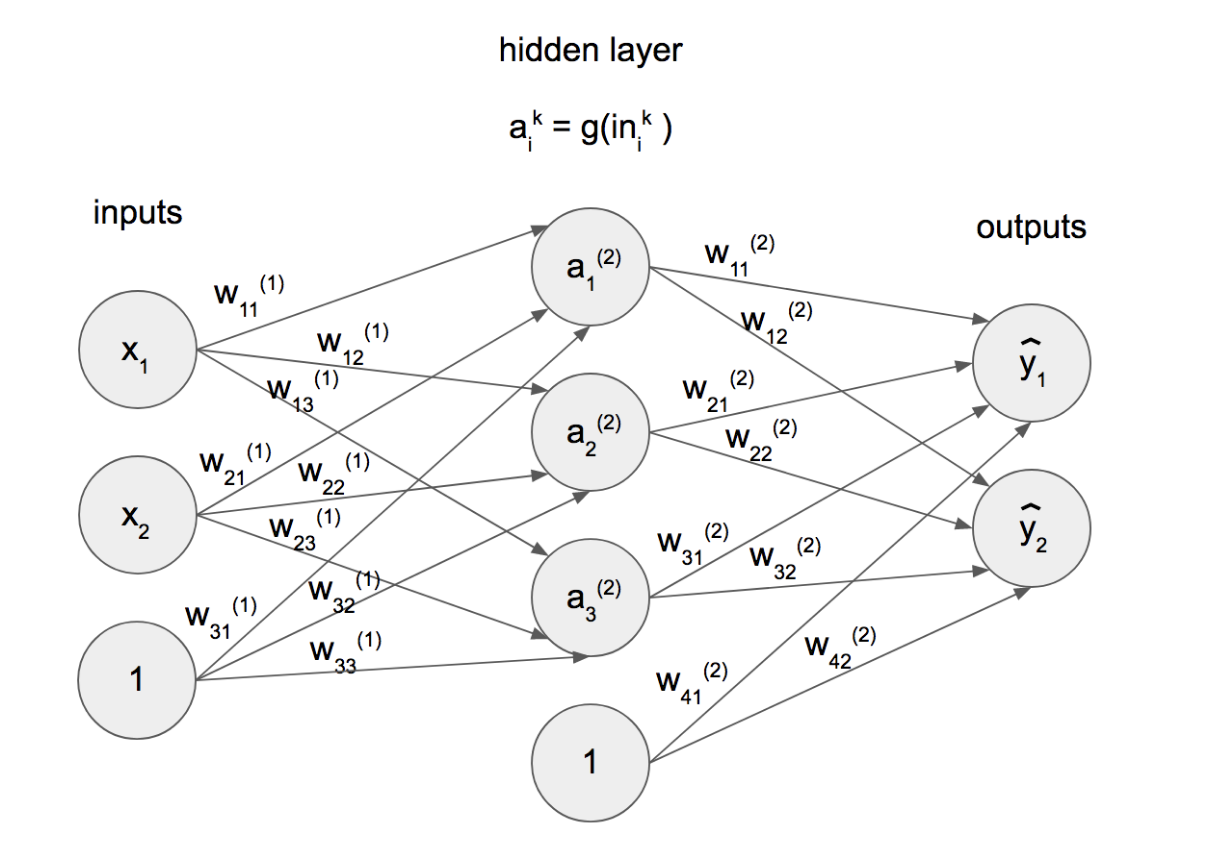
\includegraphics[width=0.7\textwidth]{activation_net}
\centering
\caption{Updated model of simple neural network from \autoref{fig:no_activation_net}. $g$ is a sigmoid activation function. Outputs are often normalized using softmax.}
\label{fig:activation_net}
\end{figure}

\begin{equation} \label{eq:sigmoid}
g(x) = \frac{1}{1 + e^{-x}}
\end{equation}

\begin{equation} \label{eq:softmax}
s(z)_j = \frac{e^{z_j}}{\sum_{k=1}^Ke^{z_k}}
\end{equation}
Softmax function $s(z)_j$ “squashes” a $K$-dimensional vector $z$ to $K$-dimensional probability distribution, where $j=1, ..., K$.\\

The goal of neural network's learning process is to find correct weights, i. e. weights, that will result in a mathematical model, where the difference of inputs is clearly represented in the difference of output vectors, which are subjects to analysis and prediction. For example in a trained dog breed classifier, the output vector for an image of german shepherd is clearly different than for york's. This can be easily interpreted and lead to correct human-readable prediction of a breed. Currently, the best known way to train a network is via algorithm called backpropagation. Main idea of this method is to calculate gradients of a cost function E (e. g. categorical cross entropy) with respect to each of weights, which are later updated by some portion of these gradients as illustrated in \autoref{eq:update_rule}.

\begin{equation} \label{eq:update_rule}
w_{ij}^{'(k)} \leftarrow w_{ij}^{(k)} - \alpha\frac{\partial E}{\partial w_{ij}^{(k)}}
\end{equation}
where:
\begin{itemize}
\item[$\alpha$] is a learning rate (indicating what portion of gradient should be used).
\end{itemize}

Let us consider a neural network in \autoref{fig:simple_net} with three units, one hidden layer and sigmoid activation function. Before conducting backpropagation, so called, forward pass was performed, which simply is a mathematical inference of outputs, given inputs (\autoref{eq:inference}).\\

\begin{figure}[h]
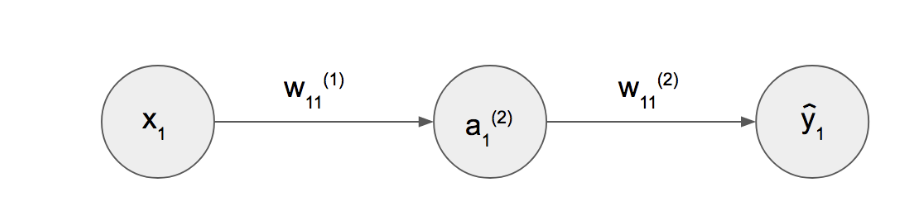
\includegraphics[width=0.6\textwidth]{simple_net}
\centering
\caption{A simple neural network, with sigmoid activation function $g$ (\autoref{eq:sigmoid}), i. e. $a_1^{(2)}=g(w_{11}^{(1)}x_1)$.}
\label{fig:simple_net}
\end{figure}

\begin{equation} \label{eq:inference}
\hat{y_1} = \frac{w_{11}^{(2)}}{1 + e^{-w_{11}^{(1)}x_1}}
\end{equation}

As mentioned previously, NN's learning algorithm is based on calculating partial derivatives with respect to each of weights. A deep nesting of functions, representing more complicated networks, encourages to make use of chain rule \cite{chain_rule_def}. \autoref{fig:backprop} outlines a single step of backpropagation using categorical cross entropy error function $E$. \autoref{eq:gradient_1} and \autoref{eq:gradient_2} present symbolic gradient calculations, necessary for learning process to occur. At this point, a beautifully simple derivative of sigmoid function is worth recalling:
\[ s'(x) = \frac{\partial}{\partial x}\frac{1}{1 + e^{-x}}\]
\[s'(x) = \frac{e^{-x}}{(1 + e^{-x})^2} \]
\[s'(x) = \frac{1}{1 + e^{-x}} * \frac{e^{-x}}{1 + e^{-x}}\]
\[ s'(x) = s(x)(1 - s(x))\]

\begin{figure}[h]
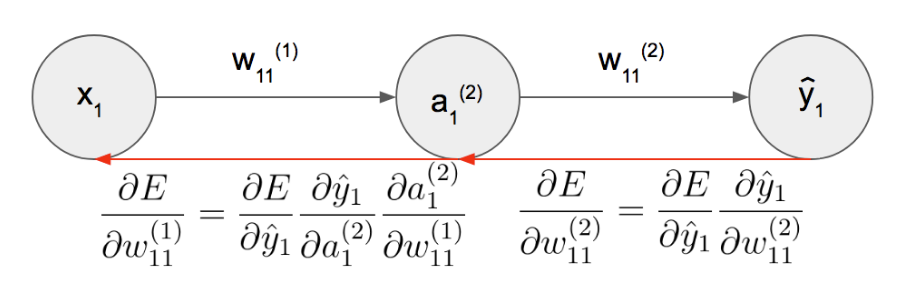
\includegraphics[width=0.55\textwidth]{backprop}
\centering
\caption{Outline of a single step of backpropagation with chain rule, where $E=-y_1log(\hat{y_1})$. Value $y_1$ is a desired binary output from training set.}
\label{fig:backprop}
\end{figure}

\begin{equation} \label{eq:gradient_1}
\frac{\partial E}{\partial w_{11}^{(2)}} = - \frac{y_1}{ln(10) * \hat{y_1}(1 + e^{-w_{11}^{(1)}x_1})}
\end{equation}

\begin{equation} \label{eq:gradient_2}
\frac{\partial E}{\partial w_{11}^{(1)}} = - \frac{w_{11}^{(2)}y_1x_1e^{-w_{11}^{(1)}x_1}}{ln(10) * \hat{y_1}[(1 + e^{-w_{11}^{(1)}x_1})^2]}
\end{equation}

With symbolic computations behind, consider following inputs to neural network from \autoref{fig:backprop}:
\begin{enumerate}[1)]
\item $x_1=10, y_1=1$ - a training example. NN should strive for returning 1, via variable $y_1$, whenever the input is equal to 10.
\item $w_{11}^{(1)}=0.3, w_{11}^{(2)}=0.5$ - randomly initialized weights for first forward pass (\autoref{eq:inference}).
\end{enumerate}
Primary step of learning process is performing inference, given randomly initialized weights and input. The produced outcome is $\hat{y_1} \approx 0.48$, which is quite far from desired 1 ($y_1$). Backward pass allows to calculate gradients with respect to each weight, namely $\frac{\partial E}{\partial w_{11}^{(2)}} \approx -0.86,  \frac{\partial E}{\partial w_{11}^{(1)}} \approx -0.2$. After applying update rule from \autoref{eq:update_rule}, with learning rate $\alpha=0.5$, new weights are $w_{11}^{(1)} \approx 0.4, w_{11}^{(2)} \approx 0.93$ and produce outcome $\hat{y_1} \approx 0.91$(much closer to desired 1). Presented algorithm is iterative. With increased amount of repetitions of above step and larger amount of examples, it should converge to optimal weights (globally or locally).
\clearpage

\section{Introduction to Convolutional Neural Networks} \label{introduction_to_cnns}
In \autoref{fig:input} a reader can see a common representation of a grayscale image, depicting number 7 in low resolution (4x4). Supplying these pixel values as a vector input of size 16 to a regular neural net, detecting if number 7 is present in a picture or not (\autoref{fig:regular_net_image}), could yield a desired result, but with a huge cost. All inputs must be mapped to each hidden neuron, hence the amount of weights will grow drastically for even slightly higher image resolution. Additional pitfall is a complete loss of spatial connections between pixels, which are essential during object recognition. The solution involves introduction of local connectivity. Consider breaking a picture from \autoref{fig:input} into four regions as in \autoref{fig:segmented_input}. Then, each hidden node could be coupled with only the pixels from one of these regions as \autoref{fig:cnn_column} and \autoref{fig:cnn_spacial} show. This simple idea is utilized in convolutional neural networks (CNNs/ConvNets) and will assist during further comprehension of this chapter.

\begin{figure}[h]
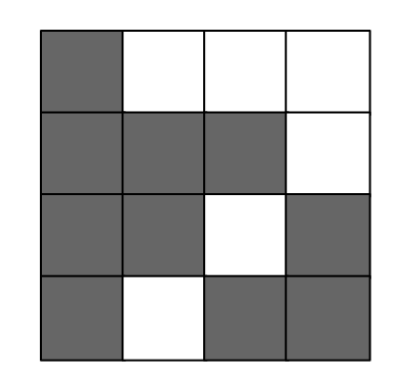
\includegraphics[width=0.3\textwidth]{input}
\centering
\caption{Grayscale image of number 7 (4 x 4 pixels resolution).}
\label{fig:input}
\end{figure}

\begin{figure}[h]
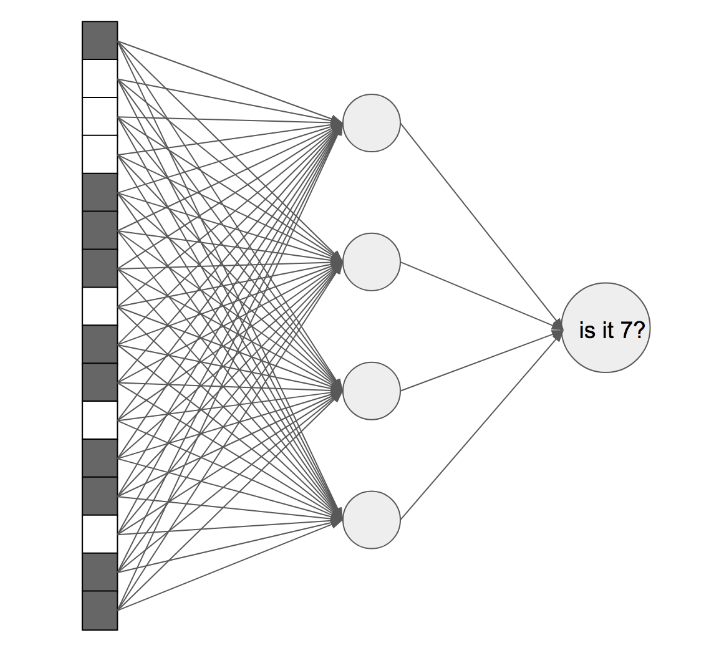
\includegraphics[width=0.5\textwidth]{regular_net_image}
\centering
\caption{Regular neural network recognizing number 7 in image input from \autoref{fig:input}, which is deconstructed (flattened) into vector of size 16.}
\label{fig:regular_net_image}
\end{figure}

\begin{figure}[h]
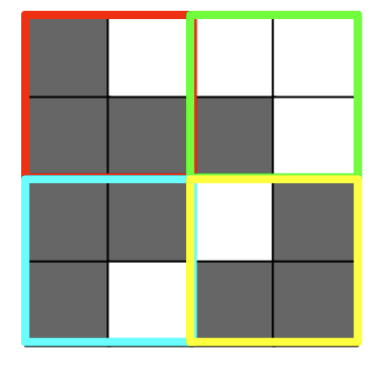
\includegraphics[width=0.3\textwidth]{segmented_input}
\centering
\caption{A number from \autoref{fig:input} divided into four pixel regions.}
\label{fig:segmented_input}
\end{figure}

\begin{figure}[h]
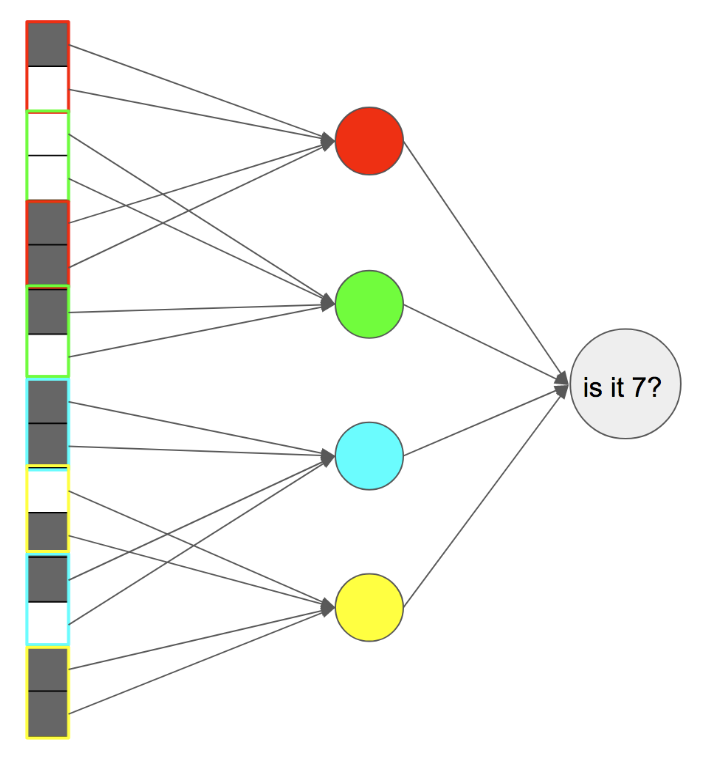
\includegraphics[width=0.5\textwidth]{cnn_column}
\centering
\caption{Local connectivity of inputs from \autoref{fig:segmented_input} to hidden nodes (vector form).}
\label{fig:cnn_column}
\end{figure}

\begin{figure}[h]
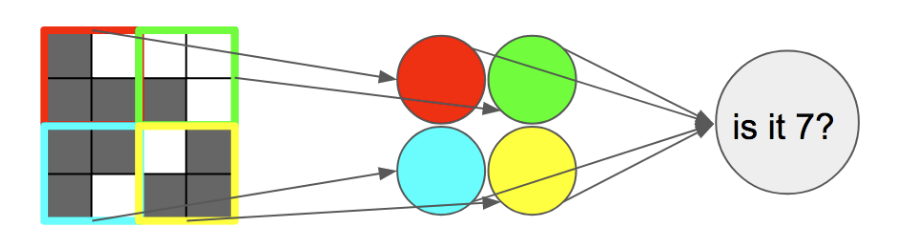
\includegraphics[width=0.5\textwidth]{cnn_spacial}
\centering
\caption{Local connectivity of inputs from \autoref{fig:segmented_input} to hidden nodes (matrix form).}
\label{fig:cnn_spacial}
\end{figure}

The standard reference for ConvNets is \textit{"Object Recognition with Gradient-Based Learning"} by LeCun et al. (1999) \cite{lecun_object}. This section attempts to explain 2 most basic building blocks of the system designed in that paper, called LeNet-5 (\autoref{fig:lecun_net}), which are:
\begin{enumerate}[1)]
\item convolutional layer,
\item subsampling layer.
\end{enumerate}

\begin{figure}[h]
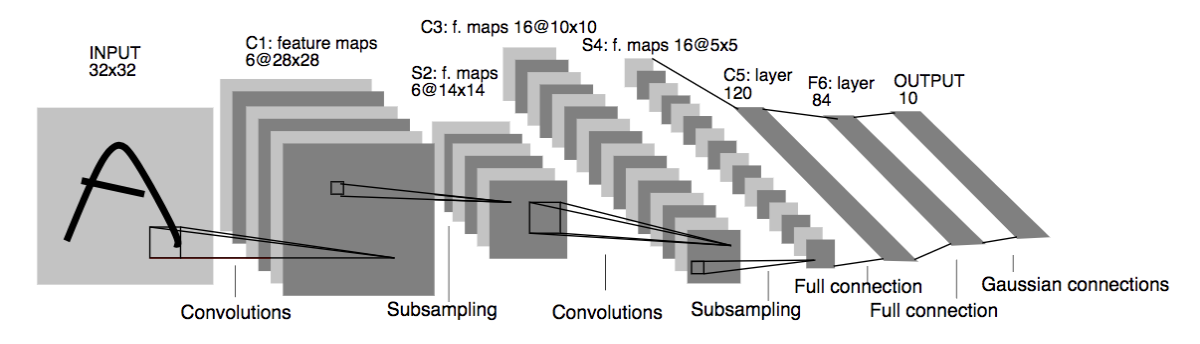
\includegraphics[width=0.8\textwidth]{lecun_net}
\centering
\caption{LeNet-5 CNN \cite{lecun_object} used for handwritten digit recognition.}
\label{fig:lecun_net}
\end{figure}

Ad 1. Filter (also called convolution window) is a tool for obtaining convolutional layer. In essence, it's a matrix with coefficients (weights), which slides, with a certain stride, over previous layer (in \autoref{fig:convolution} the previous layer is an input layer) and performs a dot product. The outcome of this operation is saved into a new matrix, called a feature map. A collection of features maps (in case of \autoref{fig:convolution} a single feature map) is called a convolutional layer. There are only a few major differences between simplified model above and the ones used in practice. Firstly, pixel values are non-binary, i. e. they are represented by an integer between 0 and 255, which is often normalized to fall into a real range [0, 1]. Secondly, recognition is often performed on RGB images (Red Green Blue \cite{rgb_def}). As a result of that, the size of the input is width x height x depth instead of width x height, where depth simply equals the number of color channels: 3. Convolutions are then performed simultaneously across each color matrix. Thirdly, \autoref{fig:convolution} presents only a single, atomic step constituting inference in CNNs. In next phase, the output of previous convolution (a collection of feature maps) is undergone the same process, but with a use of a different filter. And lastly, filters are often stacked together (multiple convolution windows are used at the same time). Only then, succeeding convolutional layer can possess multiple feature maps. As with regular neural networks, the goal of the learning process, using backpropagation, is to find correct weights (filter coefficients).\\

\begin{figure}[h]
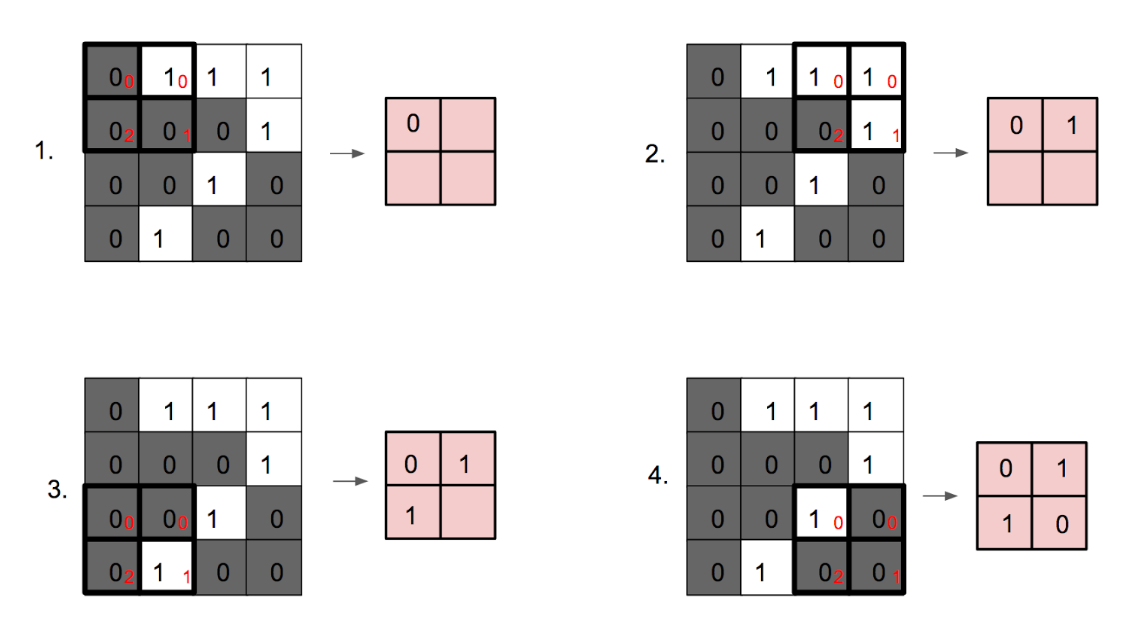
\includegraphics[width=0.8\textwidth]{convolution}
\centering
\caption{Consecutive steps of convolution using filter of size 2x2 with stride 2 (coefficients visible in red in the bottom right corner of a filter). The pink matrix is called a feature map and in this case represents a convolutional layer.}
\label{fig:convolution}
\end{figure}

Ad 2. Subsampling layers serve two purposes: reducing network dimensionality and helping it to generalize. One of the most popular subsampling techniques used today is max pooling. A window slides across a matrix with a certain stride (in a way similar to filter), takes element with the highest value and saves it to a reduced tensor (\autoref{fig:max_pooling}).\\

\begin{figure}[h]
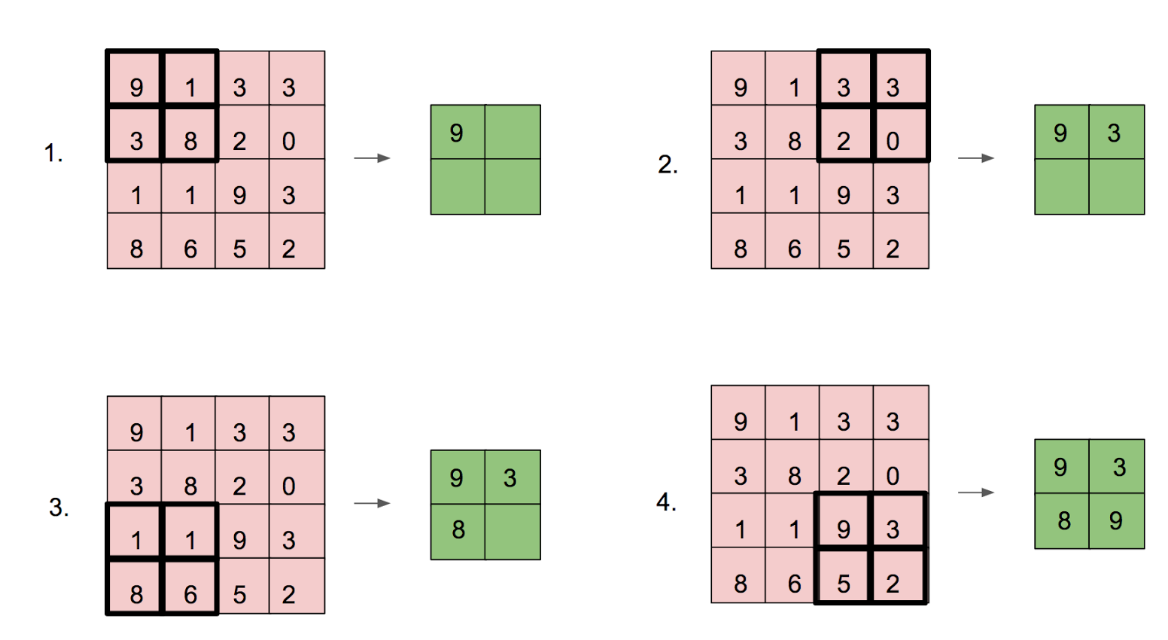
\includegraphics[width=0.8\textwidth]{max_pooling}
\centering
\caption{Consecutive steps of max pooling with window of size 2x2 and stride 2. Green matrix is a reduced tensor.}
\label{fig:max_pooling}
\end{figure}

Last thing worth mentioning is that, similarly to normal neural networks, CNNs rarely propagate activations (values of elements in features maps) explicitly to next layers. Rectifier function, also called ReLU (\autoref{eq:relu}), is often used instead.

\begin{equation} \label{eq:relu}
f(x) = max(0, x)
\end{equation}
\clearpage

\section{Comparison of world-class CNN architectures} \label{comparison_ccn_archs}
Convolutional neural networks, described in the previous chapter, take significant amount of training data to achieve high level accuracy. It is not uncommon, for more complicated recognizing tasks, to require hundred thousands of labeled images. One of the websites, which hosts such data, is ImageNet. As of November 4, 2017, it contains 14197122 images with 21841 synsets (i. e. groups of synonyms helping with information retrieval \cite{synset_def}). However, the greatest merit of ImageNet is hosting ILSVRC competition, that gave rise to CNNs, which are now considered world-class. One of the tasks of the competition is to implement an algorithm capable of recognizing 1000 different objects and drawing bounding boxes around them, given 1.2 million training images. Canziani et al. \cite{canziani_analysis} noticed, that because of the competition's focus solely on accuracy, other metrics, important for practical applications, are neglected. In \autoref{fig:world_cnns} a reader can see a comparison of the most popular ILSVRC entries in the last years, which provides information about:
\begin{enumerate}[1)]
\item Top-1 accuracy - obtained by checking if the top class (the one with the highest probability in the output vector of ConvNet) is the same as target label.
\item Operations - number of operations required for inference of a single image. Linearly related to the time of a single image classification process.
\item Parameters - illustrated by circle size. The amount of neural network’s parameters i. e. the size of NN or a measure of how complicated a model is.
\end{enumerate}
Furthermore, authors of the comparison used standardization not only by task and training set, but also by hardware used: "All experiments were conducted on a JetPack-2.3 NVIDIA Jetson TX1 board (nVIDIA): an embedded visual computing system with a 64-bit ARM A57 CPU, a 1 T-Flop/s 256-core NVIDIA Maxwell GPU and 4 GB LPDDR4 of shared RAM." \cite{canziani_analysis}.

\begin{figure}[h]
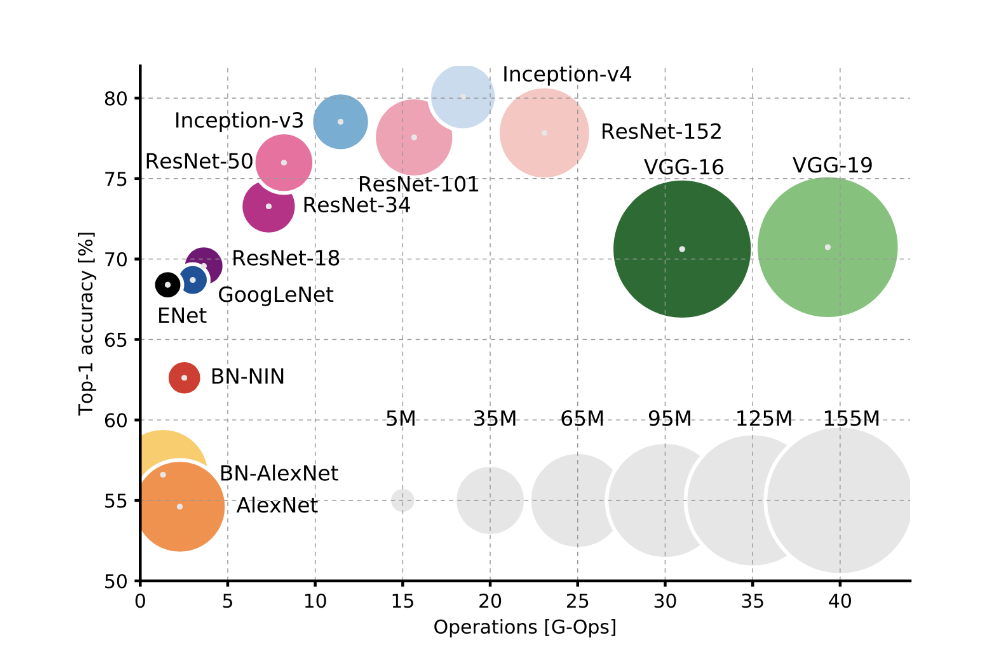
\includegraphics[width=0.7\textwidth]{world_cnns}
\centering
\caption{Comparison of world-class CNN architectures \cite{canziani_analysis} including: top-1 accuracy, number of operations and parameters.}
\label{fig:world_cnns}
\end{figure}
\clearpage

\section{Transfer learning} \label{transfer_learning}
The state-of-the-art CNN architectures, mentioned previously, are result of extensive experimentation, hyperparameters tuning, many years of expertise and months of dedicated hard work. They were based on ImageNet database and often took weeks to train. How then, could one adapt those advanced architectures to own classification tasks? The answer lies in technique called transfer learning (TL). In essence, TL is used for merging two neural networks: one, that is quite accurate at some task (e. q. everyday object recognition) and the other, which is mediocre (e. g. 5\% accuracy at beer label recognition). Thanks to the nature of the connection, a worse NN uses expertise of the better one, thus increasing own accuracy. This chapter focuses on the most common type of transfer learning, that is given a small data set, which is similar to the one advanced CNN was trained on.\\

Transfer learning step by step:
\begin{enumerate}[1)]
\item Slice off the last fully connected layer of advanced neural network, that you base TL on (\autoref{fig:tl_sliced_net}).
\item Perform inference of your entire training set, using advanced NN with sliced layer and pre-trained weights, ending up with, so called, bottleneck features i. e. a tensor image representations created by a given CNN (\autoref{fig:obtain_bottleneck}).
\item Perform training on your second (mediocre) neural network using labeled bottleneck features as inputs (\autoref{fig:using_bottleneck}).
\end{enumerate}
Above technique could differ depending on below cases:
\begin{enumerate}[a)]
\item small data set, which is different than the one advanced CNN was trained on,
\item large data set, which is similar to the one advanced CNN was trained on,
\item large data set, which is different than the one advanced CNN was trained on.
\end{enumerate}

\begin{figure}[h]
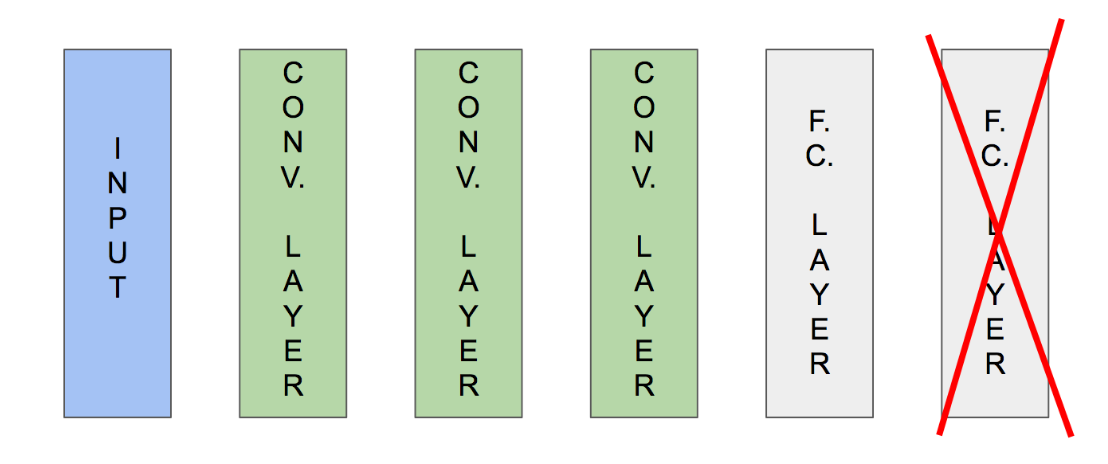
\includegraphics[width=0.8\textwidth]{tl_sliced_net}
\centering
\caption{Advanced CNN without last fully connected layer.}
\label{fig:tl_sliced_net}
\end{figure}

\begin{figure}[h]
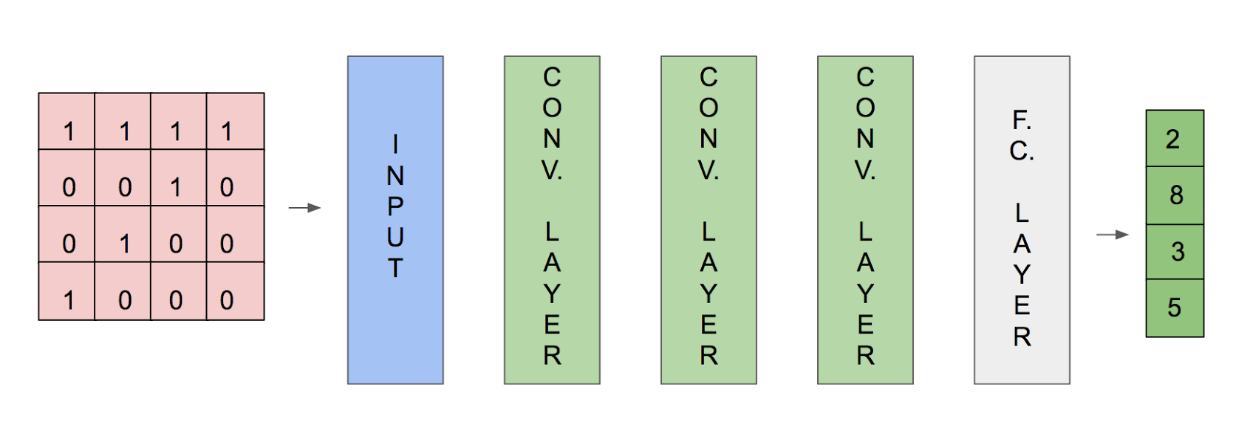
\includegraphics[width=\textwidth]{obtain_bottleneck}
\centering
\caption{Inference of one image (pink matrix) from training set using advanced CNN with sliced layer and pre-trained weights. The output (green vector) is a bottleneck feature i. e. this CNN's representation of a given image.}
\label{fig:obtain_bottleneck}
\end{figure}

\begin{figure}[h]
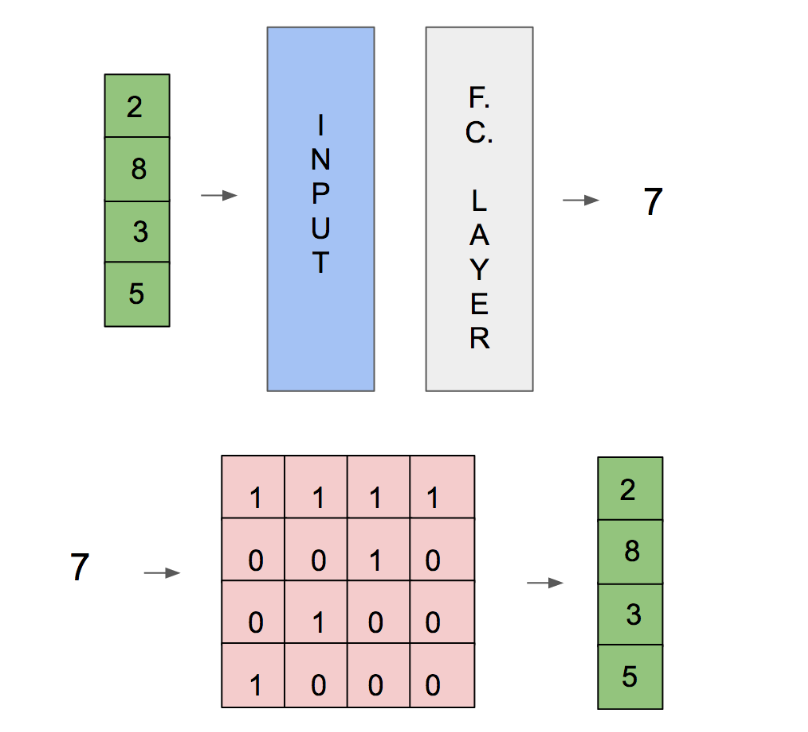
\includegraphics[width=0.6\textwidth]{using_bottleneck}
\centering
\caption{Inference in second (mediocre) neural network used in transfer learning, which is trained on labeled bottleneck features, with labeling illustrated below.}
\label{fig:using_bottleneck}
\end{figure}
\clearpage

\section{Data augmentation} \label{data_augmentation}
One can deduce, from previous introduction chapters, that an important requirement for achieving accurate machine learning models is a lot of data. Whereas for more general recognition tasks World Wide Web is a place to search for training images, the more specific the task the higher possibility of manual data collection. In that case, data augmentation is a helpful technique, allowing to artificially inflate small data set by applying a series of transformations and saving result as a new picture. \autoref{fig:augm_ex} presents exemplary augmentation of a single picture of STOP sign, yielding 10 additional training data points.

\begin{figure}[h]
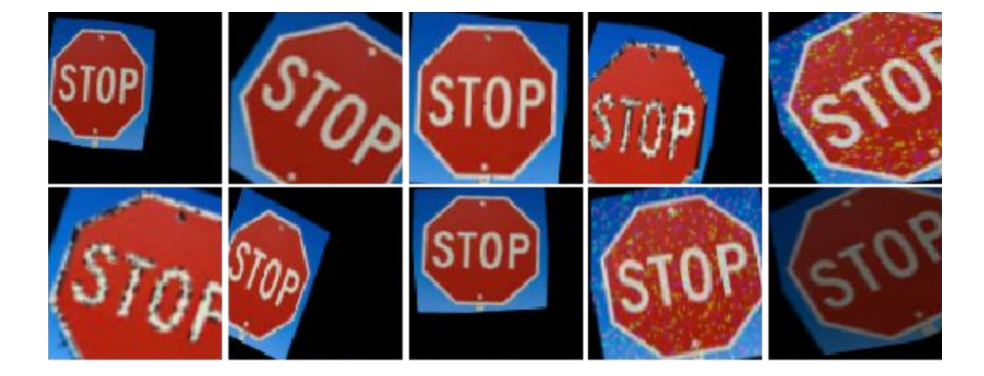
\includegraphics[width=0.7\textwidth]{augm_ex}
\centering
\caption{Data augmentation applied on a single STOP sign image.}
\label{fig:augm_ex}
\end{figure}

Transformations performed on images using data augmentation include:
\begin{enumerate}[a)]
\item changing brightness - involves converting images from RGB color space to HSV \cite{hsv_def} and adjusting V value,
\item adding noise - imposition of Gaussian noise,
\item blurring - again, Gaussian blur is oftentimes used,
\item rotation - within specific angle range,
\item translation - within specific distance range,
\item shearing - displacement of each image point, according to \autoref{eq:horizontal_shear} and \ref{eq:vertical_shear}, resulting in distortion.
\end{enumerate}

\begin{equation} \label{eq:horizontal_shear}
(x', y') = (x + my, y)
\end{equation}
Formula for horizontal shear of points in 2D space.

\begin{equation} \label{eq:vertical_shear}
(x', y')=(x, mx +y)
\end{equation}
Formula for vertical shear of points in 2D space.
\clearpage

\section{Solution walkthrough} \label{solution_walkthrough}
Focus of this chapter is reexamination of \autoref{fig:scheme}, with emphasis on used technology and implementation details.

\begin{enumerate}[1)]
\item Client application (Android).\\
This part is a basic interface used for user-server communication. The app has ability to take pictures, using built-in system camera, and then send them to server via software library called Retrofit \cite{retrofit_repo} with a popular RxJava adapter \cite{rxjava_repo}. The application is written in Kotlin programming language, which, as of mid 2017 \cite{kotlin_blogpost}, is officially supported on Android by Google. Kotlin turned out to be much more effective, expressive and less verbose alternative to Java, with which it is interoperable.

\item Beer database (Firebase).\\
This part is a database with beer information, which is sent to Android application after successful recognition. It resides on Google's NoSql cloud server \cite{nosql_def}. Data is stored as JSON and can be retrieved using very intuitive key-value query system. Despite being simple to launch and maintain, Firebase Realtime Database has currently very poor support for partial query searching, which is very anticipated in the upcoming releases.

\item Server with label classifier (Flask).\\
This part is a web server, with trained convolutional neural network, acting as beer label classifier. It is implemented in Flask - a Python microframework used for launching REST \cite{rest_def} servers. The endpoint responsible for prediction is called "/predict" and requires an image file from the caller (e. g. Android application). "/predict" obeys REST standard by using two HTTP methods: GET (as it returns encoded prediction of beer) and POST (as it accepts image file from client as input).

\item Trained convolutional neural network from Flask server.\\
This part is a CNN responsible for beer label recognition on Flask server. To create training data set, 2 - 3 pictures of labels were collected per beer. Then data augmentation technique was used, resulting in 300 - 450 images per class. Applying transfer learning created connection between two neural networks - the "worse" one, which is presented in \autoref{fig:worse_net} and the "better" one - Inception-V3 - chosen from \autoref{fig:world_cnns}, due to its small size, quick inference and relatively high accuracy. Entire procedure was implemented using Keras library with TensorFlow backend (in Python programming language). Next chapter provides reader with detailed metrics about obtained ConvNet. 
\end{enumerate}

\autoref{fig:app}, \ref{fig:firebase_data} and \ref{fig:terminal_server} partially illustrate aforementioned recognition system components.

\begin{figure}[h]
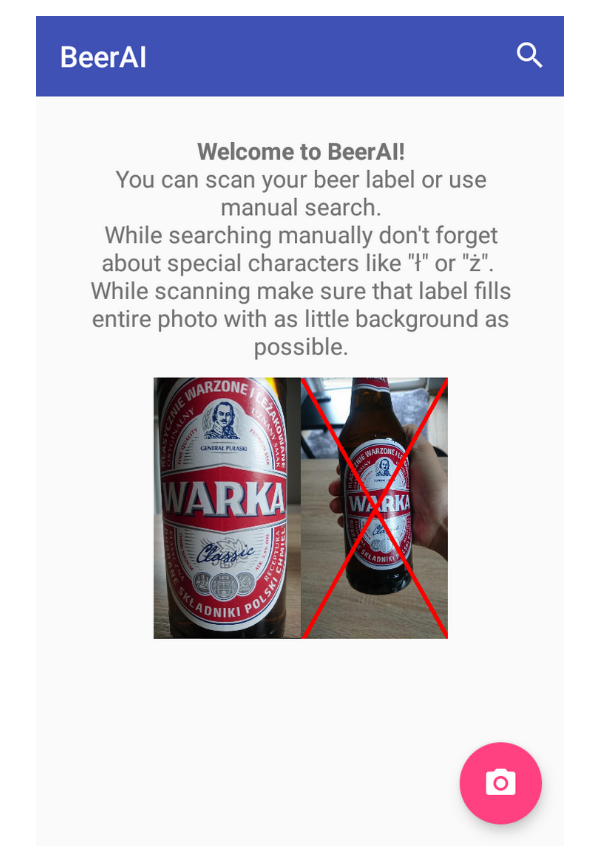
\includegraphics[width=0.4\textwidth]{app}
\centering
\caption{Main screen of Android application. Note the hints given to the user, resulting from prototype's limitations, namely: poor support of advanced searching in Firebase Realtime Database and high risk of wrong prediction given beer label image with a lot of background.}
\label{fig:app}
\end{figure}

\begin{figure}[h]
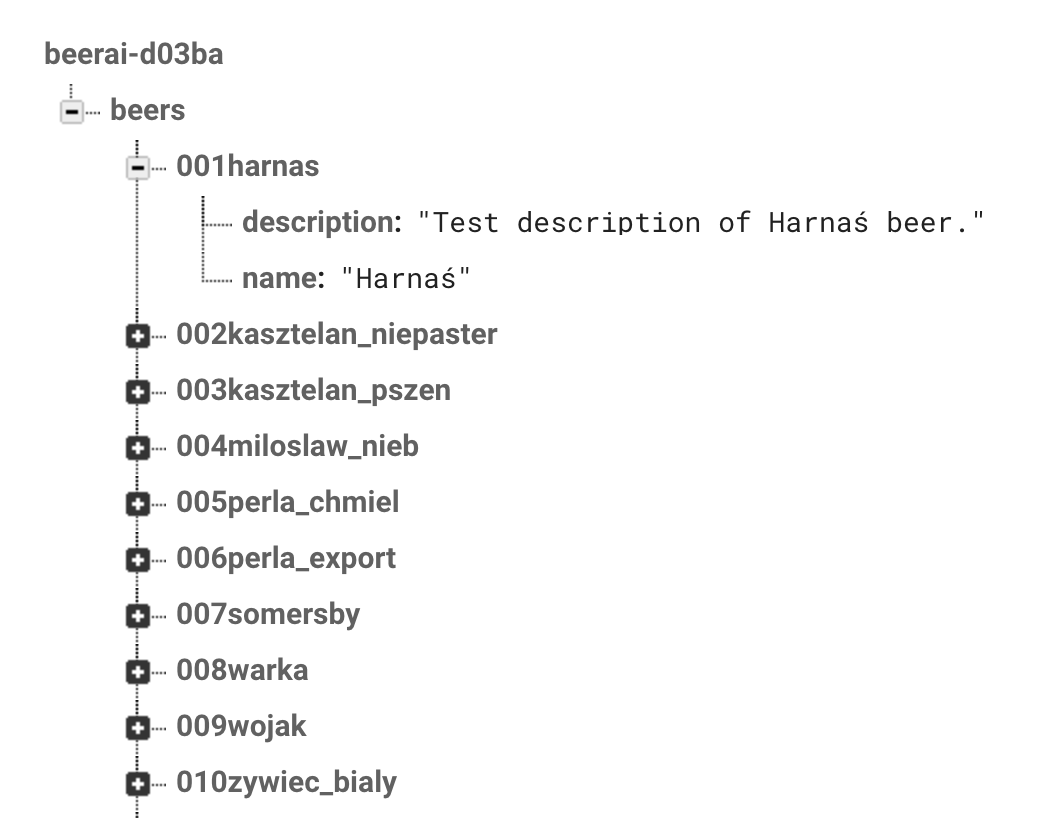
\includegraphics[width=0.4\textwidth]{firebase_data}
\centering
\caption{Firebase Realtime Database with encoded key-value pairs of beer information.}
\label{fig:firebase_data}
\end{figure}

\begin{figure}[h]
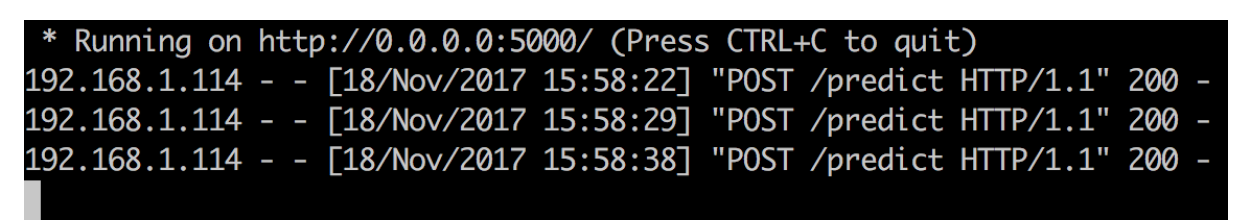
\includegraphics[width=\textwidth]{terminal_server}
\centering
\caption{Terminal view of requests sent to Flask server (to "/predict" endpoint) from Android application. "200" return code indicates that request succeeded.}
\label{fig:terminal_server}
\end{figure}

\begin{figure}[h]
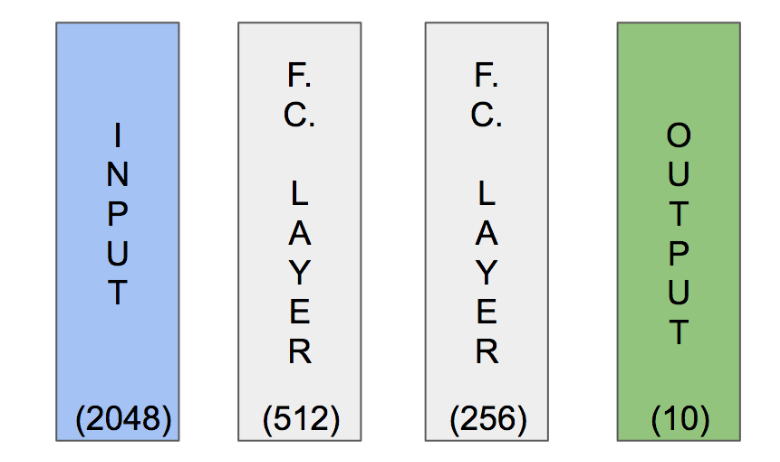
\includegraphics[width=0.5\textwidth]{worse_net}
\centering
\caption{Regular fully-connected neural network, which accuracy increased due to transfer learning based on Inception-V3. Values in brackets represent amount of neurons in each layer. Whereas number of neurons in hidden layers (f. c. layers) is fixed, inputs and outputs depend, respectively, on size of bottleneck features coming from Inception-V3 and number of beers CNN can recognize (in basic version of prototype it's 10). Both hidden layers use ReLU activation function.}
\label{fig:worse_net}
\end{figure}
\clearpage

\section{Testing} \label{testing}
Purpose of this chapter is to provide reader with metrics related to the convolutional neural network used in the prototype, which is the base of this thesis. Those metrics will be later utilized for system evaluation. All experiments were conducted on 3.1 GHz Intel Core i5 CPU with 16 GB 2133 MHz LPDDR3 RAM.\\

\autoref{fig:collected_labels} presents manually collected data set for one class. Augmentation, applied on this beer label, resulted in 150 additional pictures per image, i. e. 302 images total for \foreignlanguage{polish}{Harnaś} beer, and took on average 256.91 seconds to complete. Similar procedure was employed for remaining 9 beer labels. \autoref{fig:augm_subset} contains a small portion of augmented training set. Picture transformations used:
\begin{enumerate}[a)]
\item changing brightness - for every piece of data (using HSV color model),
\item adding Gaussian noise - 20\% probability of happening,
\item Gaussian blurring - 20\% probability of happening,
\item rotation - for every piece of data (max angle value: 90 deg),
\item translation - for every piece of data (in both directions),
\item shearing - 25\% probability of happening.
\end{enumerate}

\begin{figure}[h]
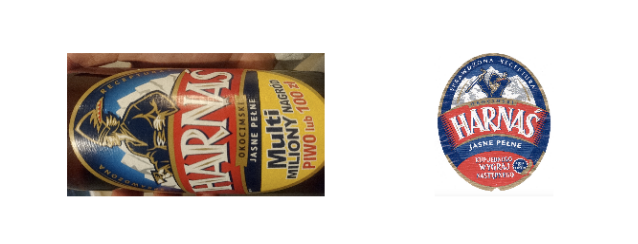
\includegraphics[width=0.5\textwidth]{collected_labels}
\centering
\caption{Manually collected data set for \foreignlanguage{polish}{Harnaś} beer label class. The first picture (2160 x 3840 pixels resolution) was taken by camera and the second one (ideal) was found on the internet.}
\label{fig:collected_labels}
\end{figure}

\begin{figure}[h]
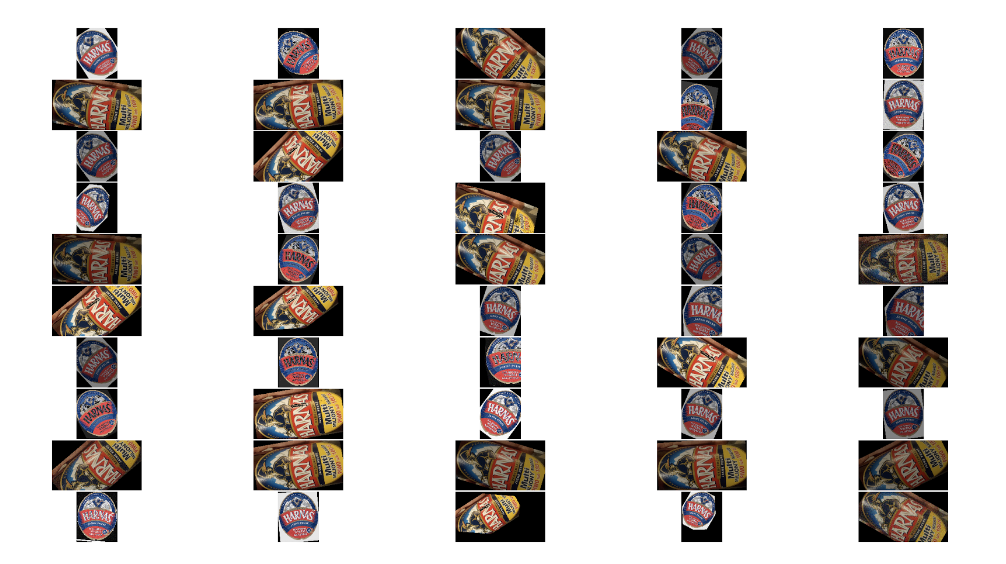
\includegraphics[width=0.6\textwidth]{augm_subset}
\centering
\caption{Small portion of augmented training set for \foreignlanguage{polish}{Harnaś} beer label class.}
\label{fig:augm_subset}
\end{figure}

Bottleneck features were extracted, using Inception-V3 neural network, for 3020 training images of all beer labels, that the prototype is capable of recognizing. At the same time, each picture underwent a dimension reduction to 150 x 150 pixels resolution and value rescaling to real range [0, 1]. This procedure took 428.19 seconds for entire data set.\\

Categorical cross entropy error function was used during training. Number of epochs (learning iterations) was set to 50, while weights were being updated after backward pass on batches of size 48. To validate accuracy a validation set of beer labels images was created, independently from the training one, and fed to obtained ConvNet (over 100 validation pictures). \autoref{fig:10_class_acc} and \ref{fig:10_class_err} contain charts of training progression, which in the end took 767.3 seconds for 10 classes and resulted in learning a total of 9571594 parameters.

\begin{figure}[h]
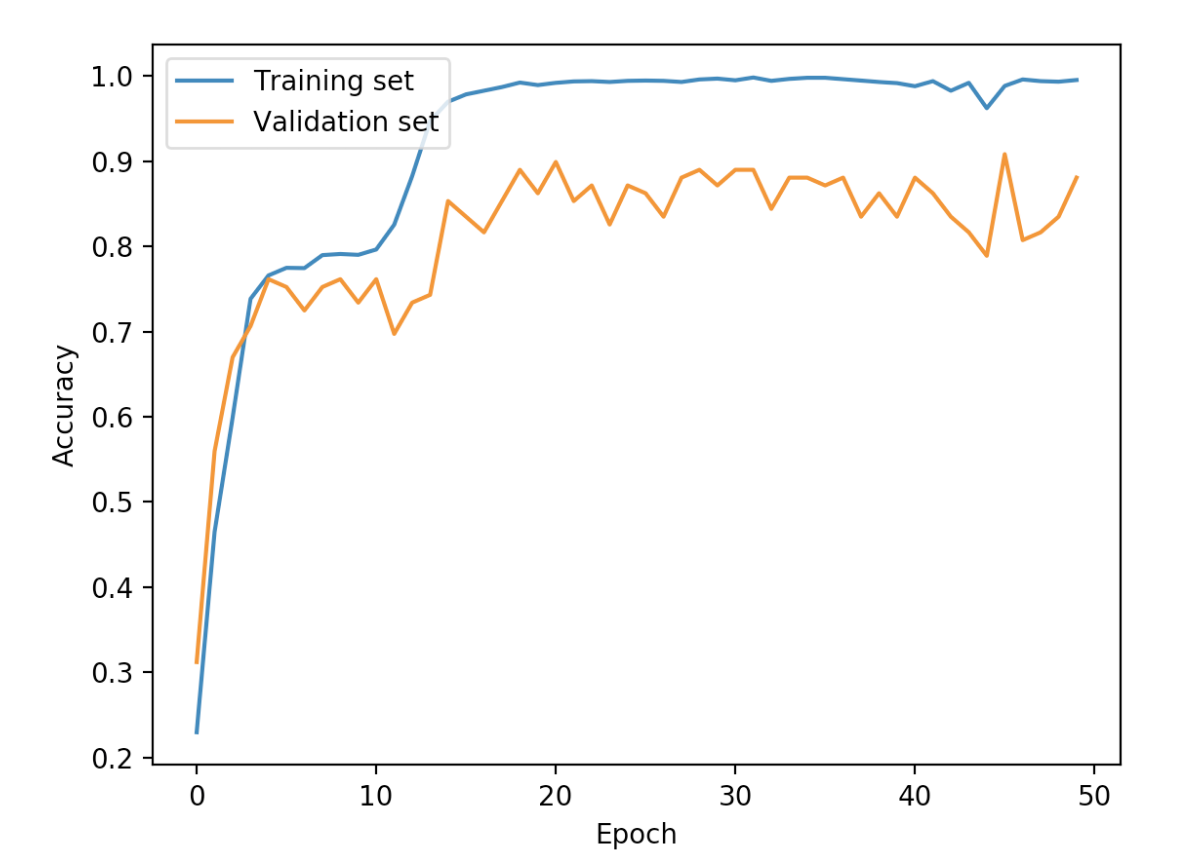
\includegraphics[width=0.55\textwidth]{10_class_acc}
\centering
\caption{Accuracy of 10-class model during training. The best obtained value is 99.5\% for training set and 89.1\% for validation set.}
\label{fig:10_class_acc}
\end{figure}

\begin{figure}[h]
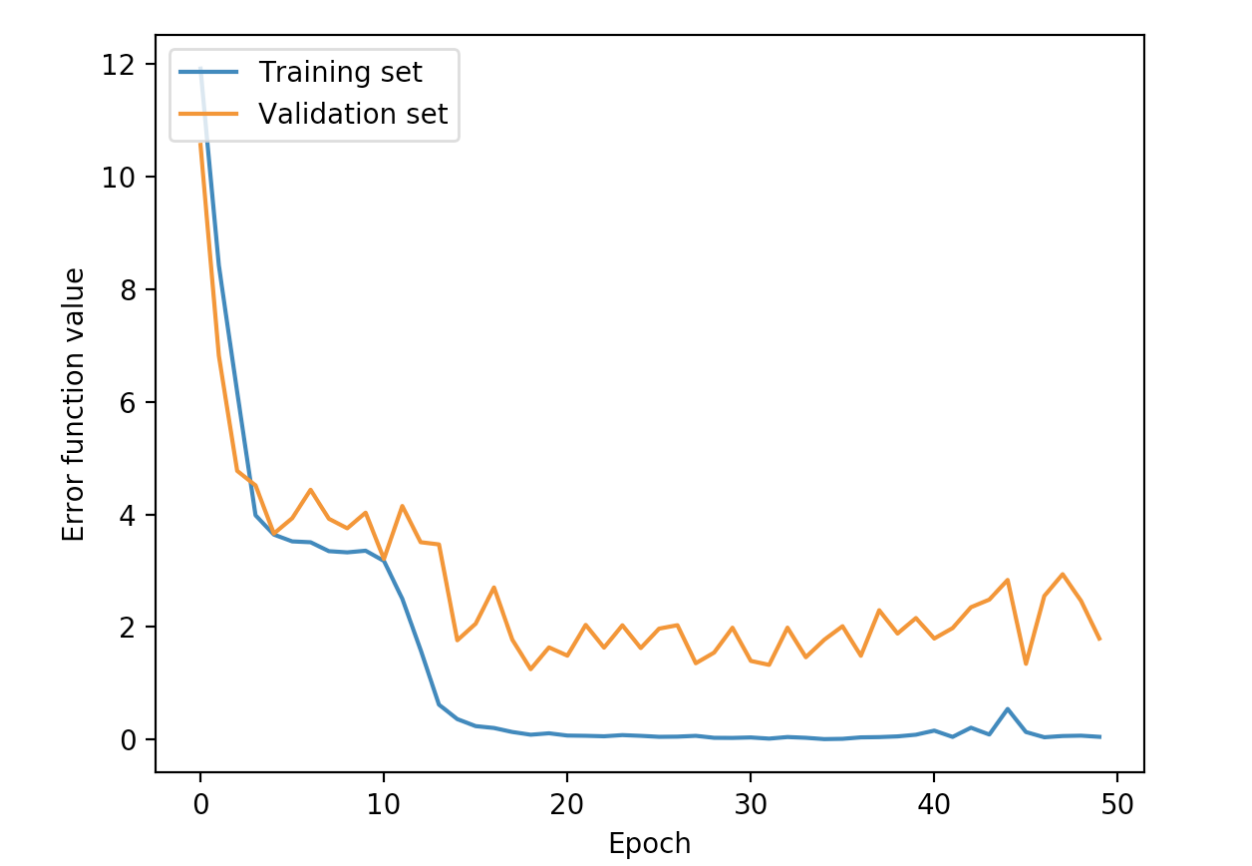
\includegraphics[width=0.6\textwidth]{10_class_err}
\centering
\caption{Categorical cross entropy error during training of 10-class CNN. The best obtained value is 0.051 for training set and 1.796 for validation set.}
\label{fig:10_class_err}
\end{figure}

Average time of a single beer label recognition, out of 10 classes, is 0.1 second. Implemented CNN was tested in different lighting conditions and with or without visible background in input image. \autoref{fig:test_table} accumulates outcomes of these tests.\\

\begin{figure}[h]
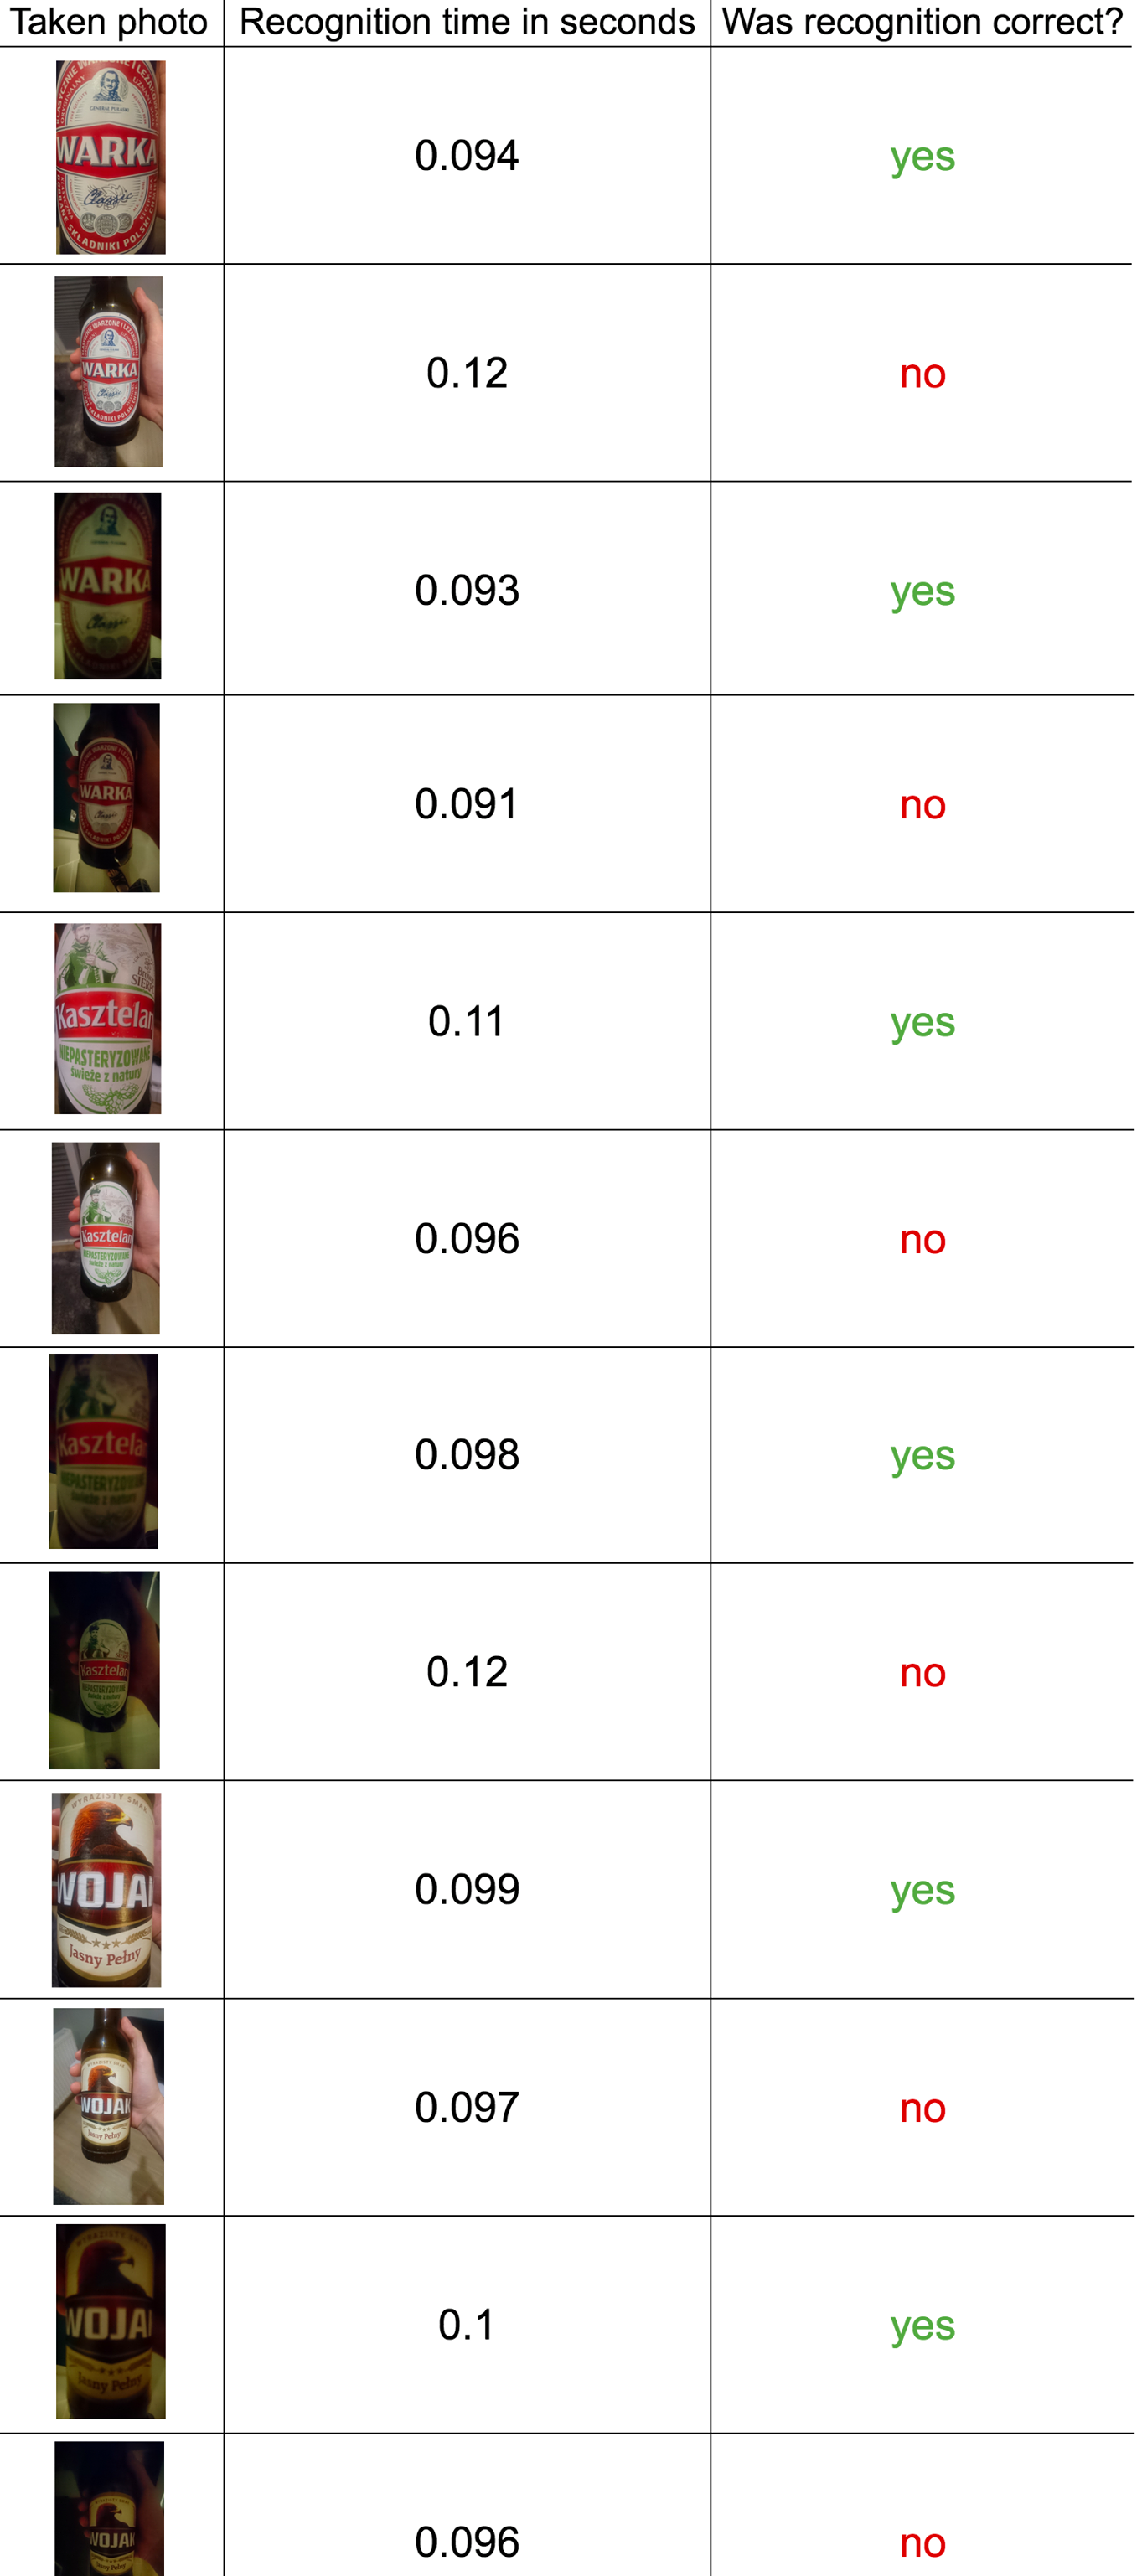
\includegraphics[width=0.4\textwidth]{test_table}
\centering
\caption{Test results for 10-class CNN (different lighting conditions and background visibility of input image).}.
\label{fig:test_table}
\end{figure}

Test for algorithm's scalability involved incorporating additional 10 classes (10 different beer labels) and retraining. Average time of a single beer label recognition, this time out of 20 classes, is 0.098 second. \autoref{fig:20_class_acc} and \ref{fig:20_class_err} contain charts of training progression, which in the end took 1253.84 seconds and resulted in learning a total of 9574164 parameters.

\begin{figure}[h]
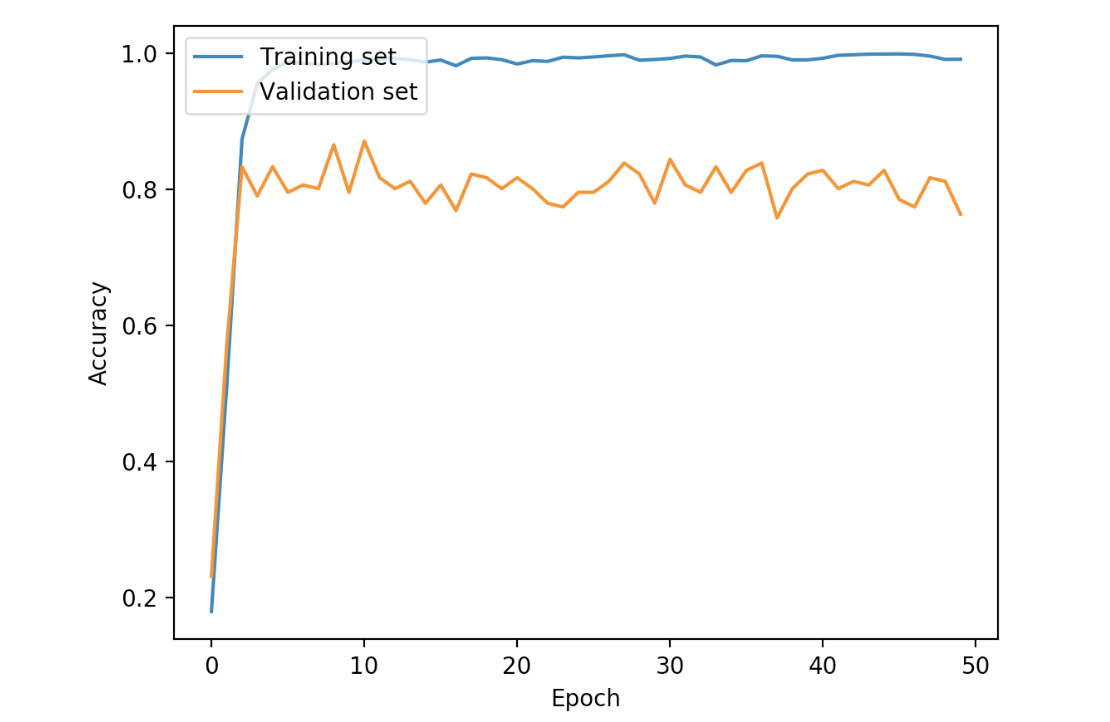
\includegraphics[width=0.7\textwidth]{20_class_acc}
\centering
\caption{Accuracy of 20-class model during training. The best obtained value is 99.8\% for training set and 87.6\% for validation set.}
\label{fig:20_class_acc}
\end{figure}

\begin{figure}[h]
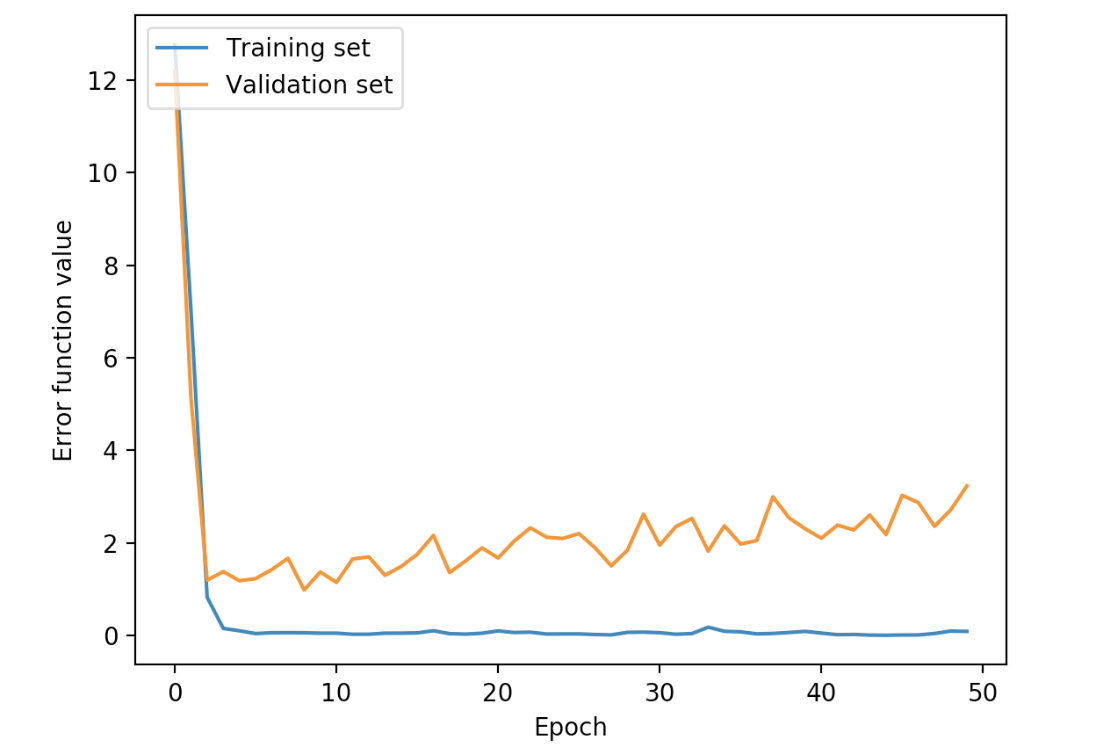
\includegraphics[width=0.7\textwidth]{20_class_err}
\centering
\caption{Categorical cross entropy error during training of 20-class CNN. The best obtained value is 0.017 for training set and 1.16 for validation set.}
\label{fig:20_class_err}
\end{figure}
\clearpage

\section{Related solutions} \label{related_solutions}
To assess a value of the proposed solution to acceleration of access to beer database problem, a research into available related techniques was conducted. It is worth noting that there seems to be no popular and continuously maintained application solving the issue using deep learning. 

\begin{enumerate}[1)]
\item SIFT algorithm.\\
Scale-Invariant Feature Transform algorithm was first described by Lowe in 1999 \cite{lowe_sift} and was used for beer label recognition by Weitz et al. at Stanford University \cite{beer_sift}. The technique extracts local features from image and later uses them for classification. SIFT proved to be robust to uniform scaling, orientation and illumination changes. It is, however, protected by patent (additional costs). Lowe's algorithm is considered mathematically complicated and computationally heavy. Each beer label identification using this solution took about 10 seconds on 8 parallel processors in MATLAB (again, more computational power imposes more costs). SIFT is included in popular OpenCV library.
\item Bar code and QR code scanners.\\
Ohbuchi et al. \cite{barcode_mobile} presented methods capable of very effective code scanning using mobile devices, which are now used across many fields for fast data retrieval. The amount of information stored in such codes is limited and defined by global norms (e. g. 1D bar code obeying Code 39 standard is advised not to contain more than 25 characters, while QR code limits are much higher - up to 1520 alpha numeric characters). Untappd is a social beer drinking mobile app, which uses bar code scanning to access its database. Despite this technique being very reliable and accurate, it creates a challenge of staying up to date with all bar code changes implemented by brewery, that oftentimes take place during some promotional campaigns. Bar code scanning also requires user to physically search for bar codes on a bottle and lacks the "fun" factor of image-based searches. QR codes are still not widely used for product identification.
\item OCR.\\
Vivino is a mobile application with access to world's largest wine database. Its algorithm used for obtaining data is based on Optical Character Recognition, namely, keywords are being extracted from wine label photo and used as an input to app's search engine. The highest costs in Vivino's approach are associated with a need to incorporate third party OCR provider (e. g. ABBYY) and creation of database supporting advanced partial searching. 
\item Custom image recognition API provider.\\
Vize.ai is an example of service allowing to easily create custom neural network to recognize specific images. It abstracts all complexity related to designing own CNN, training and uploading it to remote server. On the contrary, one of the cognitive purposes of this thesis was to delve into image recognition complexities and to obey MVP rules (Minimum Viable Product) articulated, among others, by Ries \cite{lean_startup}, hence third party recognition provider was not taken under consideration.
\end{enumerate} 
\clearpage

\section{Conclusions} \label{conclusions}
The evolution in customers' taste and their openness to local breweries resulted in a huge variety of beers available in popular Polish stores like Lidl or Carrefour. Despite this fact, customers still find it cumbersome to choose which product to buy.\\

When faced with a mobile app with beer database, users consider it the most attractive to access beer details by making a photo of front beer label. Scanning bar code seems to be the least popular.\\

Artificial Intelligence (deep learning in particular) incorporated in a mobile application can itself be a driving force behind rapid growth rate of users, following the likes of Shazam.\\

Recent increase in performance of GPUs and data available on the Internet provide a fertile ground for machine learning algorithms, such as neural networks.\\

Currently, the best way to train a neural network is by using a backpropagation algorithm. It is also utilized in CNNs, which are specialized in image recognition (they preserve spatial connections between pixels).\\

Thanks to ILSVRC competition hosted by ImageNet, many world-class CNN architectures emerged. It is particularly important because of the technique called transfer learning, which allows to adapt them to custom recognition tasks.\\

The more specific the task the higher possibility of manual data collection. However, instead of manually collecting thousands of images per class, one can artificially inflate training set by using data augmentation (applying a series of picture transformations).\\

Firebase Realtime Database, which contains data about beers, has currently very poor support for searching. The use of it excluded possibility of OCR implementation, which requires a solid partial query search engine.\\

Flask proved to be small and reliable framework for REST API creation. The prototype runs the server in the local network, however uploading it to Cloud (such as Google App Engine) is extremely easy and requires almost no additional code. \\

Implemented beer label classifier can achieve at least 87\% accuracy under user-friendly conditions, with inference time not exceeding 0.2 second. Aggregation of additional beer labels does not significantly change accuracy nor recognition time. It can be concluded, that drastic increase in number of classes, which CNN is capable of identifying, will result in a classifier, which inference time won't surpass 1 second, while still maintaining around 90\% success rate. \\

There seems to be no popular and continuously maintained application solving beer label recognition problem using deep learning. Untappd app's developers implemented bar code scanning to accelerate beer database access. On the other hand, Vivino is using OCR but for wines only. Once popular NextGlass mobile application has not been updated since 2015. 
\clearpage

\bibliography{mybib}
\bibliographystyle{siam}

\end{document}